\begin{savequote}[75mm] 
Live long and prosper
\qauthor{Spock} 
\end{savequote}

\chapter{Machine learning based algorithm for long-lived particles reconstruction in LHCb}
\label{chapter ML algo}

This chapter presents a Machine Learning based study related to the improvement of the Downstream Tracking algorithm. It starts by providing the general introduction to the LHCb track reconstruction methodology, then the Downstream Tracking algorithm is described including a section focused on a seed classifier. Then, the performance of the entire Downstream Tracking algorithm is discussed. The final section is dedicated to present ideas on how to approach similar types of problems by leveraging more sophisticated Deep Learning models. Those model will be tested as a part of development of the Downstream Tracking algorithm for the Upgraded LHCb experiment.   

\section{Track reconstruction}
Tracking is one of the most important steps in event reconstruction. This procedure is dedicated to reconstructing particle trajectories using a collection of hits that were created when a particle interacts with tracking stations. Tracks are used to provide precision vertexing and momentum estimation. Without that information, no physics analysis can be performed. Moreover, track information together is important is crucial for particle identifi
\begin{figure}[h]
\centering
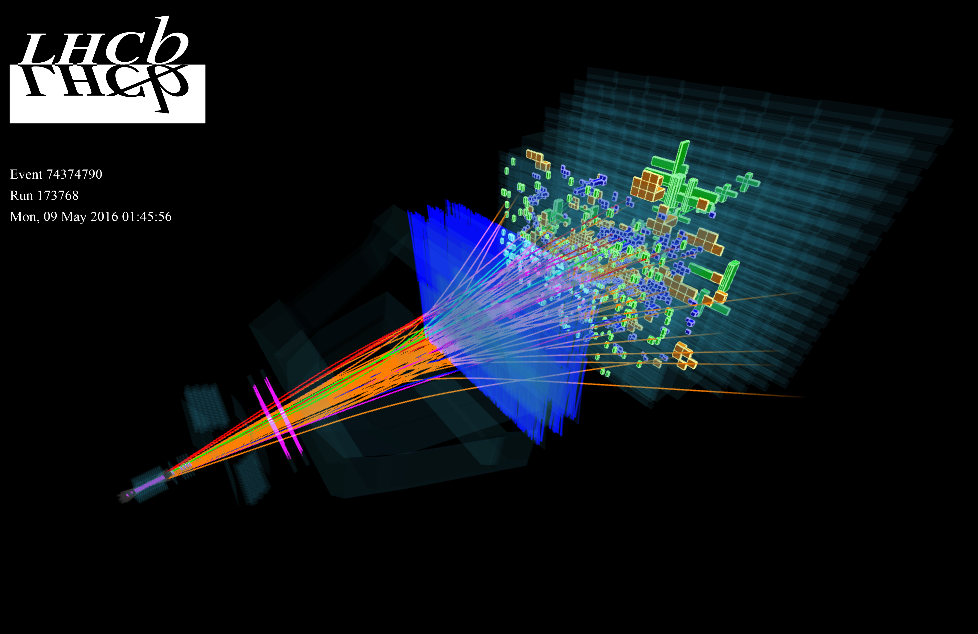
\includegraphics[scale=0.9]{figures/LHCb7_event.png}
\caption{A typical LHCb event fully reconstructed during data taking on May 9th 2016 (during Run II). Particles identified as pions, kaon, etc. are shown in different colours. Figure taken from \cite{LHCb_event_display}.
\label{fig:event display}}
\end{figure}


One of the analyses, which utilize long-lived particles is a study of time-dependent CP-violating asymmetries in $B_0 \rightarrow J/\psi K_S^0 $ decays. Measurement of time-dependent CP asymmetries provide a valuable test of the flavor sector of the Standard Model as well as an opportunity for discovery effects of physics beyond the Standard Model.  
 The study of this asymmetry in the $B_0 \rightarrow J/\psi K_S^0 $  decay mode provides a way to determinate the effective CP phase. The CP violation asymmetry in $b \rightarrow c\bar{c}s$decays of the B mesons is caused by the interference between mixed and unmixed decay amplitudes.
 A state initially prepared as a $B^0$ can directly decay into $J/\psi K_S^0$ or can oscillate into a $\bar{B}$ and then decays into  $J/\psi K_S^0$. Taking the correction to the theoretical uncertainty, this amplitude is equal to twice the angle $\beta = arg [ -  \frac{V_{cd}V_{cb}^*}{V_{td}V_{tb}^*} ] $ of the Unitary Triangle. 



\begin{figure}[h]
\centering
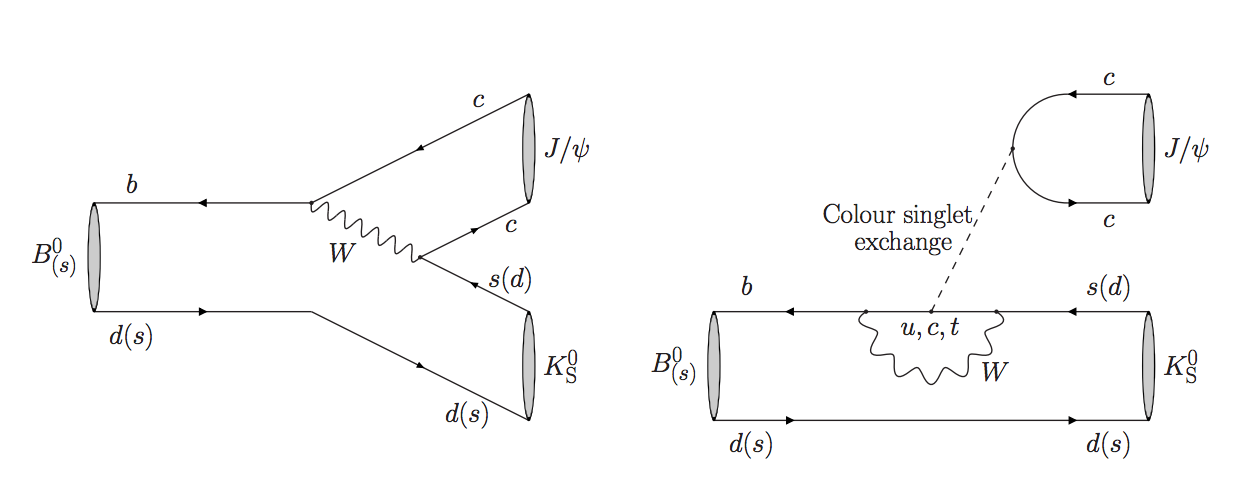
\includegraphics[scale=0.9]{figures/B0JPKs.png}
\caption{The Feynman diagram presenting the decay topologies contributing to the $B_0 \rightarrow J/\psi K_S^0 $ channel:  (left) tree diagram and (right) penguin diagram, taken from [??]
\label{fig:BJPSi}}
\end{figure}

\section{Downstream Tracking Algorithm overview}
\label{Sec:Downstrean Overview}
Downstream tracks at LHCb are reconstructed in the following way. First a standalone track reconstruction in the T stations with an algorithm called PatSeeding is performed, creating T tracks. After filtering with a Machine Learning classifier to discard bad candidates i.e. tracks that don’t represent the trajectory of a real particle, these tracks are propagated back through the magnet to the TT station, assuming they are coming from the point of origin of the coordinate system. The TT consists of four layers of silicon microstrip sensors: the first and last layer have strips running vertically (so-called x1 and x2 layers) and probe the x coordinate. The layers in between, called stereo layers, have the strips tilted by 5◦ (u layer) and $-5\degree$ (v layer), respectively. This allows for the determination of  the y coordinate. The TT is separated into two sections: TTa comprises the x1 and u layer, TTb comprises the v and x2 layers. One cluster is searched for in the two x layers of the TT. This already allows to constrain the flight path of the particle with a good precision. Then a cluster in the other x layer is searched for. Lastly, clusters are searched in the u and v layers. The clusters are then fitted with a $\chi^2$ fit using a parabola as a model. As with a bunch-crossing frequency of 25 MHz spillover can occur, a flag is set for each cluster if it is likely to have been created in a different collision than the one in question (so-called «high-threshold bit»); tracks with a large number of high-threshold clusters are rejected. Finally, the best track is chosen according to the output of another multivariate classifier. 


\section{Downstream Track model}



\subsection{Propagation through the magnetic field}
\label{sec:magPoint}
Neglecting multiple scattering, particles propagating through the tracking
stations, which all lie outside the magnetic field of \lhcb, will follow a straight
line path, and the bending of the trajectory inside the field can be
approximated by a sharp kink in the flight path at a given $z$ position of a magnet point, called $z_{\text{mag}}$ (see Fig.~\ref{fig:magnetPointSketch} for an illustration). The $z$ position of this point depends on the parameters of the track itself, and is also affected by inhomogenities in the field. The idea is to parametrize this point as precisely as possible from the properties
of the T track. The following empirical formula is used:

\begin{eqnarray}
\label{eq:zMag}
z_{\text{mag}} & = &\alpha_{0} + \alpha_{1} \cdot t_{y}^{2} + \alpha_{2} \cdot t_{x}^{2} + \alpha_{3} \cdot 1/p \\
& & +\, \alpha_{4} \cdot | x_{T} | + \alpha_{5} \cdot | y_{T} | + \alpha_{6} \cdot | t_{y} |. \nonumber
\end{eqnarray}
Here, $t_{x}$ and $t_{y}$ are the slopes of the last track state in the
T stations. The absolute momentum, $p$, is
estimated from the T track, using a parametrisation that assumes a kink of the trajectory 
at the center of the magnet and the track to come from the point of origin.
The observables $x_{T}$ and $y_{T}$ are the
$x$ and $y$ positions of the last state in the T stations, respectively. The
variable $z_{\text{mag}}$ depends most strongly on the values in the first line of
Eq.~\ref{eq:zMag}, while the dependence on the ones from the second row is
smaller.

\begin{figure}[!htbp]
 \begin{center}
    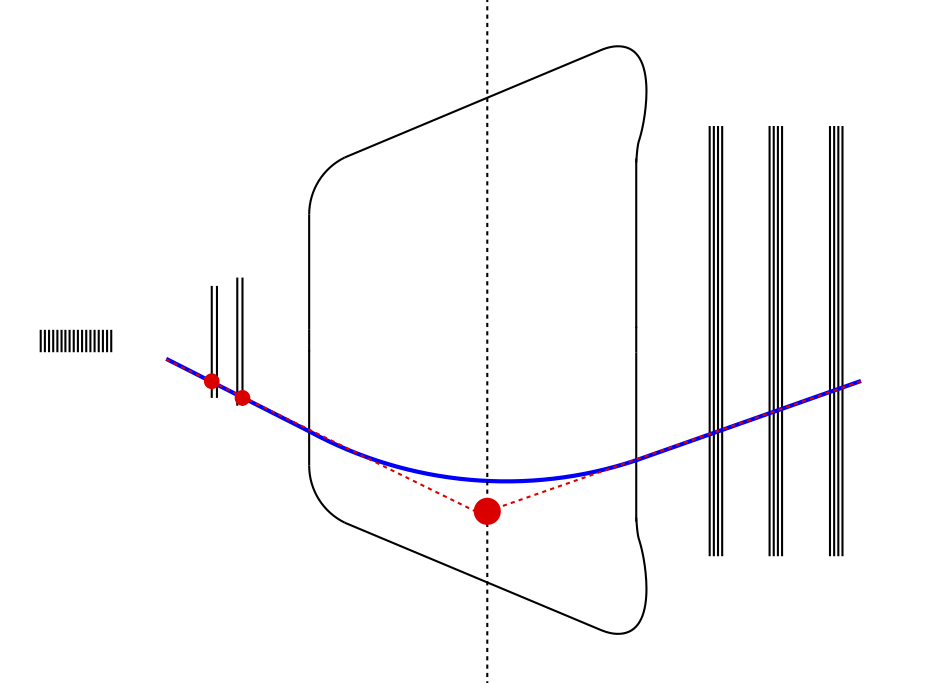
\includegraphics[width=0.49\linewidth]{figures/magnetPointDownstream2.png}
   \caption{Sketch of the LHCb detector with the tracking system in the $x$-$z$ plane. A downstream track (blue line) and its approximation outside the magnetic field (red dotted line) is shown. In the approximation the track undergoes a sharp kink at the magnet point (big red dot).
     \label{fig:magnetPointSketch}}
 \end{center}
\end{figure}

The $\alpha$ parameters are determined in simulation, by fitting a straight line to the
true position of the hits in TT, and a third order polynomial to the true
position of the hits in the T stations. The crossing point of both curves in the $x$-$z$ projection
determines the <<true>> value of $z_{\text{mag}}$. An illustration of $z_{\text{mag}}$ determined in this way, and
the difference between the values obtained with Eq.~\ref{eq:zMag} when using measured 
instead of simulated quantities are shown in Fig.~\ref{fig:zMag}.

\begin{figure}
 \begin{center}
   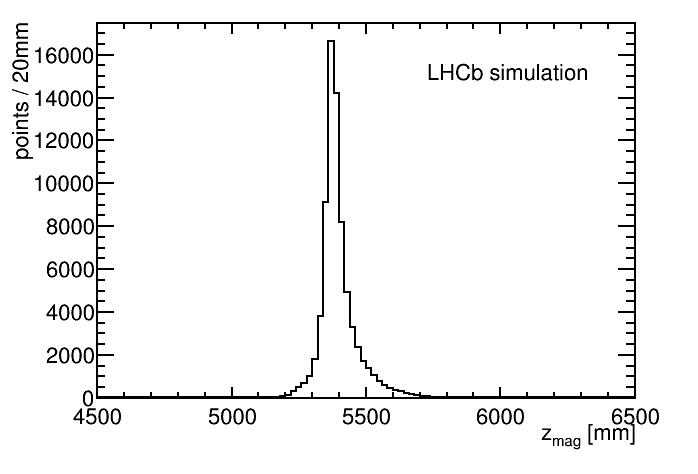
\includegraphics[width=0.49\linewidth]{figures/zMag.png}
    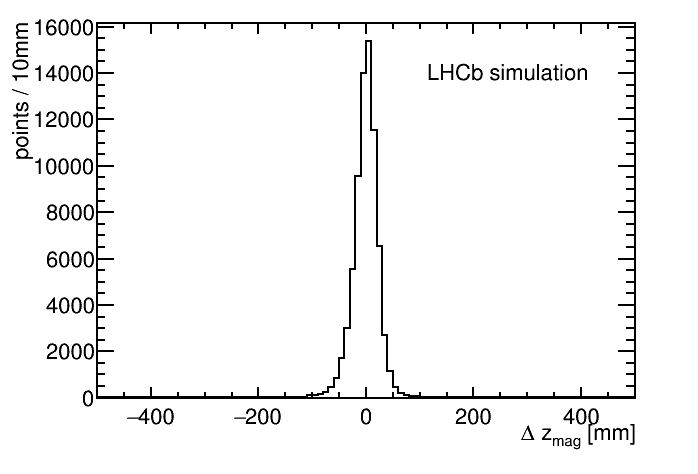
\includegraphics[width=0.49\linewidth]{figures/deltaZMag.png}
   \caption{Left: <<True>> z position of the magnet point. Right: Difference
   between true and estimated $z$ position of the magnet point. For the true position, simulated observables, for the estimated position measured observables were used.
     \label{fig:zMag}}
 \end{center}
\end{figure}

The $x$ position of the magnet point is then determined by extrapolating the
state in the T stations linearly to $z_{\text{mag}}$.
\begin{equation}
x_{\text{mag}} = x_{T} + t_{x} \cdot (z_{\text{mag}} - z_{T})
\end{equation}
For the $y$ position, an additional correction is applied:

\begin{equation}
\label{eq:ymag}
y_{\text{mag}} = y_{T} + t_{y} \cdot (z_{\text{mag}} - z_{T}) - \beta_{1} \cdot t_{y} \cdot \Delta_{\text{slope}}^{2}
\end{equation}
with $\Delta_{\text{slope}}$ the difference of the slopes in $x$ before and after the magnet, determined as
\begin{equation}
\Delta_{\text{slope}} = \left| x_{\text{mag}}/z_{\text{mag}} - t_{x} \right|,
\end{equation}
and $\beta_{1}$ an empirical parameter, determined on simulation, to correct
for the effect of the magnetic field on the $y$ position.
The predicted slope in $y$ in the TT is calculated as:

\begin{equation}
t_{y,TT} = t_{y} \cdot (1 + \beta_{0} |t_{y}| \Delta_{\text{slope}}^{2})
\end{equation}
with  $\beta_{0}$ an empirical parameter, determined on simulation, 
using regression with true observables, to correct
for the effect of the bending in the magnetic field on the slope in $y$.

A special treatment is needed for tracks with hits in the OT only: As the
$y$ resolution and the resolution of the slope in $y$ is rather poor, the track
is constrained to come from $y(z=0) = 0$. The following parametrisation is used:
\begin{eqnarray}
y_{TT} & = & y_{T} + t_{y} \cdot (z_{\text{mag}} - z_{T}) + t_{y,TT} \cdot (z_{TT} - z_{\text{mag}}) - \beta_{1} \cdot t_{y} \cdot \Delta_{\text{slope}}^{2},
\end{eqnarray}
with $\beta_{1}$ again determined on simulation using regression with true observables. 
Assuming that no further correction is needed between the point of origin of the
track and TT, the slope in the T stations can be calculated as:
\begin{equation}
t_{y, \text{constr}} = y_{T} / ( z_{T} + (\beta_{0} |t_{y}| z_{\text{mag}} + \beta_{1} ) \Delta_{\text{slope}}^{2})
\end{equation}

For tracks with hits in the OT only, $t_{y, \text{constr}}$ is used in
Eq.~\ref{eq:ymag} instead of the measured value $t_{y}$.

As the magnet point will be used as an additional constraint in the \chisq fit
(see Sect.~\ref{sec:chi2}), an uncertainty has to be assigned to it. This is
calculated by determining the difference between the values of $x_{\text{mag}}$ and
$y_{\text{mag}}$ obtained using simulated quantities and reconstructed quantities for
the extrapolation. The uncertainty depends on $\Delta_{\text{slope}}$ and whether the track
mainly has IT or OT hits. The following parametrisations of the uncertainty
were used:
\begin{eqnarray}
\sigma_{x, OT} & = & (2.0 + 18.0\cdot \Delta_{\text{slope}})\mm \nonumber \\
\sigma_{y, OT} & = & (5.0 + 20.0\cdot \Delta_{\text{slope}} + 50\cdot \Delta_{\text{slope}}^{2})\mm  \nonumber \\
\sigma_{x, IT} & = & (1.0 + 16.0\cdot \Delta_{\text{slope}})\mm  \nonumber \\
\sigma_{y, IT} & = & (2.0 + 15\cdot \Delta_{\text{slope}})\mm  \nonumber
\end{eqnarray}
These parameters were obtained by fitting residual distributions.

\subsection{Determination of the momentum}
The momentum of a downstream track mainly depends on the kink it undergoes in
the magnetic field, but also shows a dependence on the slopes in $x$ and $y$.
The following parameterisation results in a momentum resolution of about 2\%
averaged over the momentum spectrum.
\begin{eqnarray}
\label{eq:momentum}
p & = & \frac{ \gamma_{0} + \gamma_{1} \cdot t_{x}^{2} + \gamma_{2} \cdot t_{y}^{2} }{ \Delta_{\text{slope}} },
\end{eqnarray}
where again the parameters $\gamma_{i}$ were determined using the true position
of the hits in simulation. This resolution contains both the effect from the detector 
resolution and from dependencies which are not accounted for in the parametrization. 
The resolution is illustrated in Fig.~\ref{fig:momReso}.
\begin{figure}[!htbp]
 \begin{center}
   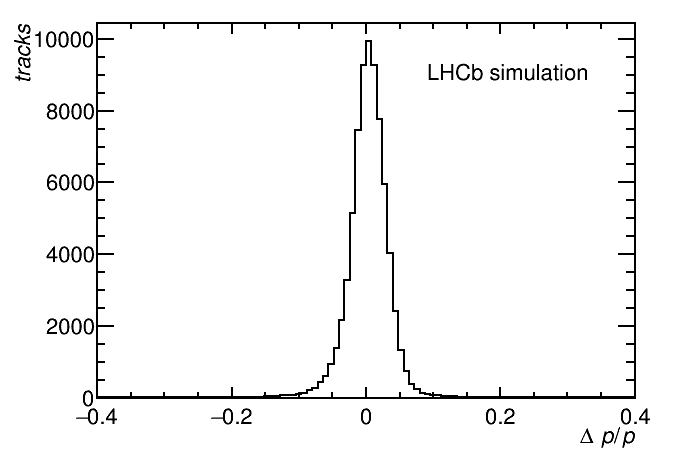
\includegraphics[width=0.8\linewidth]{figures/momReso.png}
    \caption{Momentum resolution for the initial track estimate. It amounts to about 2\%.
     \label{fig:momReso}}
 \end{center}
\end{figure}


\subsection{Track model in the TT}
\label{sec:trackModelTT}
Despite the fact that the strength of the magnetic field is greatest in the region between TT and the T stations,
there is a strong enough residual field in and before the TT such that low-momentum particles undergo deflection from a
straight line. A downstream track therefore is represented by a
parabola in the TT. However, as a parabola has three degrees of freedom, but one
has to be able to fit a track with three clusters in the TT only, the
curve-parameter is fixed from the kink of the track through the magnetic field in order for the $\chi^2/\ndf$ value from the fit to provide a meaningful goodness-of-fit statement.
The track model therefore is:

\begin{equation}
x(z) = x_{0} + t_{x} \cdot (z - z_{\text{mag}}) +c \cdot (z - z_{TT})^{2},
\end{equation}
with $z_{TT}$ the $z$ position in the middle of the TT, $z_{mag}$ the $z$
position of the magnet point, $t_{x} $ the slope in $x$ in TT, and
$c= 1.48\cdot 10^{-5} \cdot \Delta_{\text{slope}}$. The initial value for $x_{0}$ is $x_{\text{mag}}$. 
The parameter $c$ is determined on
simulation by fitting the true position of the hits in TT with a parabola
and determining it as a function of $\Delta_{\text{slope}}$. The deflection from a
straight line is very small: for a track with a momentum of 3\gevc it is about
200\mum, which is about the strip pitch of a TT sensor.

The initial slope in $x$ of the track in TT is given by:
\begin{equation}
t_{x,TT} = x_{\text{mag}}/z_{\text{mag}}.
\end{equation}
As explained in Sect.~\ref{sec:magPoint} the slope in $y$ is given by:
\begin{equation}
t_{y,TT} = t_{y} \cdot (1 + \beta_{0} |t_{y}| \Delta_{\text{slope}}^{2})
\end{equation}
with $t_{y}$ being replaced by $t_{y, \text{constr}}$ in the case of a track with OT
hits only. Note that $t_{y}$ is not updated in the fit (see Sect.~\ref{sec:chi2}). 
The function for the $y$ position therefore is:

\begin{equation}
y(z) = y_{0} + t_{y,TT} \cdot (z - z_{\text{mag}}),
\end{equation}
where the initial value for $y_{0}$ is $y_{\text{mag}}$. 

\section{Pattern Recognition}

This section provide an overview of the stages of the pattern recognition in LingLivedTracking, which are presented in the figure \ref{fig:PatLL}. The detailed description on the first step, filtering T seeds, was moved into the separate section  \ref{sec:TSeed}. 

\begin{figure}
\centering
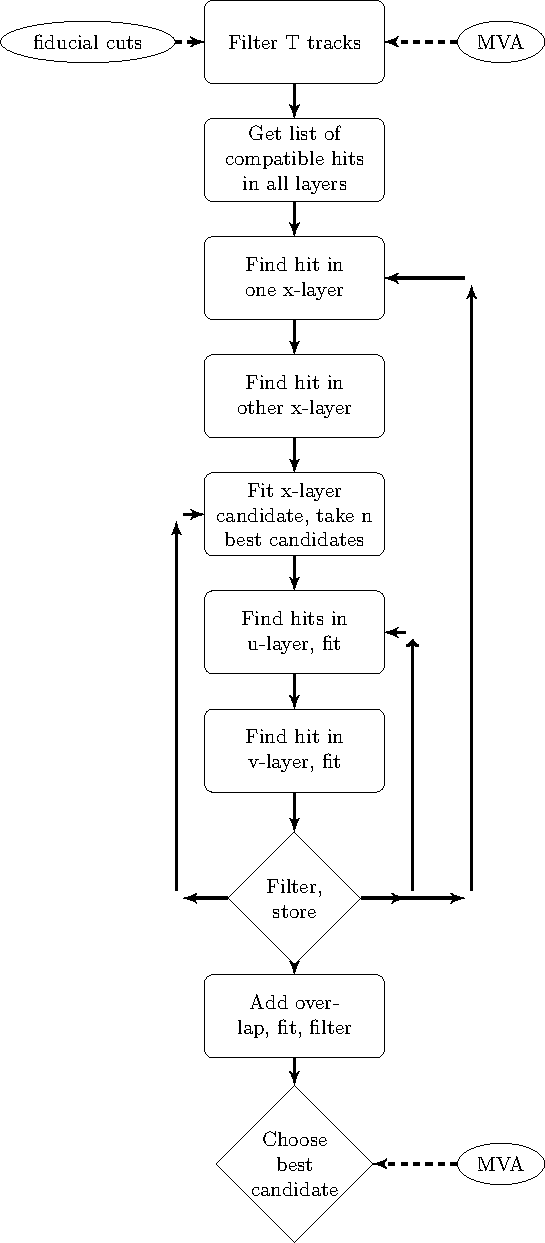
\includegraphics[scale=0.7]{figures/PatLL.pdf}
\caption{Different stages of pattern recognition within the  PatLongLivedTracking algorithm. 
\label{fig:PatLL}}
\end{figure}


\subsection{PatSeeding}
The algorithm, that performs pattern recognition for the T-seeds is called PatSeeding. It consists of five distinct steps: 

\begin{itemize}
\item hit preparation;
\item track search per detector region;
\item track search for tracks migrating from IT to OT;
\item track search per Outer Tracker region for tracks at large $|y|$;
\item validation of low-quality tracks left over from the per region search;
\end{itemize}


Each layer of the main tracking stations is divided into six different regions. Because there
are few tracks migrating between regions, the second step is executed per detector region, thus reducing combinatorics. Within this algorithm, the track is described as a straight line particle trajectory in $x-y$ plane.  For $x-z$ projection, a cubic model with three parameters is used:
\begin{eqnarray}
x(z)&=&c(z-z_{reference})^2(1+d_{ratio}(z-z_{reference})) + b(z-z_{reference})+a \\
y(z)&=&b_{y}z+a_y
\end{eqnarray}

$d_{ratio}$ describes the correlation between the quadratic and cubic terms and is determined from
Monte Carlo studies. The shift by $z_{reference}$ makes the fit more numerically stable ($z_{reference}$ is
in the middle of the T stations, by default).

\subsection{First search for compatible hits}
Track candidates at this stage have the magnet point  (see Sect.~\ref{sec:magPoint}) as the only constrain,
 and the track model at this point is a straight line from (0,0,0) to the magnet point.
To correct for the fact that most particles of interest do not originate from
the global \lhcb origin (0,0,0), a correction to the $x$ position of the search
window is applied, which is also derived from simulation. The value is given by:

\begin{equation}
\delta x = \text{sign}(p\cdot \text{magPol}) \cdot \left( \texttt{XCorrectionConst} / p + \texttt{XCorrectionOffset} \right),
\end{equation}
with magPol the magnet polarity. An illustration can be seen in
Fig.~\ref{fig:preselWindow}, left. 
 
To search for hits compatible with this first track estimate, momentum-dependent
search windows in the TT are opened.
An illustration can be seen in Fig.~\ref{fig:preselWindow}. The
dependence of the window size on the momentum is:

\begin{equation}
\Delta x = \texttt{XPredTolConst} / p + \texttt{XPredTolOffset},
\end{equation}
where $p$ is the absolute value of the momentum. The parameters determining the
size of the search window, \texttt{XPredTolConst} and
\texttt{XPredTolOffset}, were derived on simulation, illustrated on the right of
Fig.~\ref{fig:preselWindow}.

\begin{figure}[!htbp]
 \begin{center}
  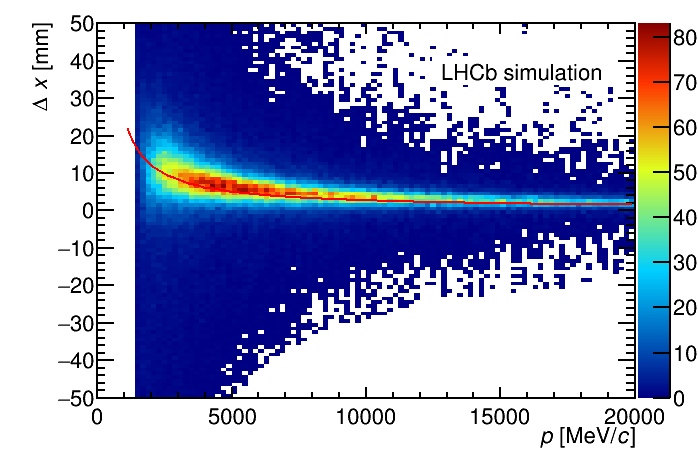
\includegraphics[width=0.49\linewidth]{figures/xPosCorrection1.png}
   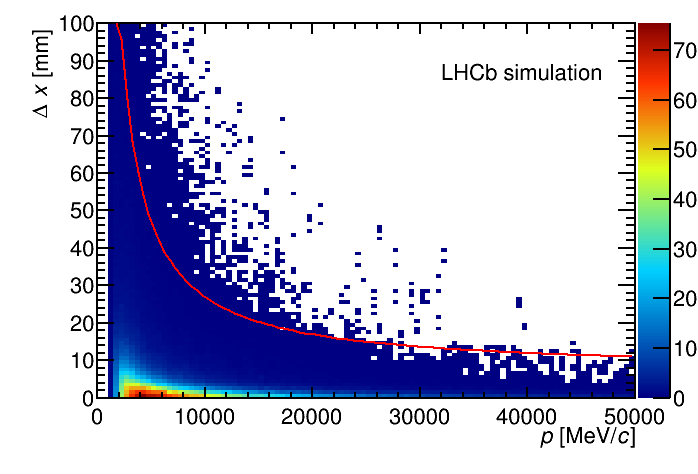
\includegraphics[width=0.49\linewidth]{figures/preselWindow1.png}
   \caption{Left: Distance between extrapolated track (constrained to come from the \lhcb origin (0,0,0)) and (truth-matched) hits
   before correction. The red line represents the correction function which is
   applied. Right: Distance between extrapolated track and (truth-matched) hits
   as a function of the momentum of the track for the preselection step, after
   the correction. The cut is show as the red line.
     \label{fig:preselWindow}}
 \end{center}
\end{figure}



Furthermore, it is checked if the hit is compatible with the expected $y$
position in the TT with a tolerance \texttt{YTol}. As the position of a hit in the TT can only be determined up to
the length of a sensor module, this provides only a weak constraint. The $x$
positions of the hits in the stereo layers are then updated, assuming the $y$
position from the T track extrapolation.

All hits in all four layers which lie inside these tolerances are then stored in a container, and
sorted according to the projection distance, \ie the absolute distance of
the hit to the predicted position.

The T track is not considered if less than 3 hits in the TT are found in
total, or the $x$ or the stereo layers do not contain any hit.

\subsection[Search for hits in $x$ layers]{Search for hits in {\boldmath $x$} layers}
In this step, the algorithm iterates over all hits in the $x$ layers.
The first hit is chosen in one of the two $x$ layers, if a hit is present. This allows for a more precise
determination of the slope of the track and the curvature, and therefore also of the momentum of
the track -- these quantities of the track candidate
are therefore updated. Next, corresponding hits in the other $x$ layer are
searched for. This essentially means that, if several hits are present in both $x$ layers, 
all possible combinations between the hits are iterated over. This leads to the duplication of hit combinations,
which however given the good timing performance of the algorithm (see Sect.~\ref{sec:timing}) is negligible.

The search window in the other $x$ layer is defined as follows:

\begin{equation}
\Delta x =  \texttt{TolMatchConst} / p + \texttt{TolMatchOffset} ,
\end{equation}
if $\Delta x$ is smaller than a given value \texttt{MaxWindowSize}, otherwise
\texttt{MaxWindowSize} is taken as the tolerance. This serves as a sanity check
to exclude unphysically large values of the window size for low momentum
particles. All hits within this window are then considered for further
processing. As illustrated in the left hand plot of Fig.~\ref{fig:matchingDist}, 
essentially all hits from true particles
in simulation are enclosed within this region.

\begin{figure}[!htbp]
 \begin{center}
  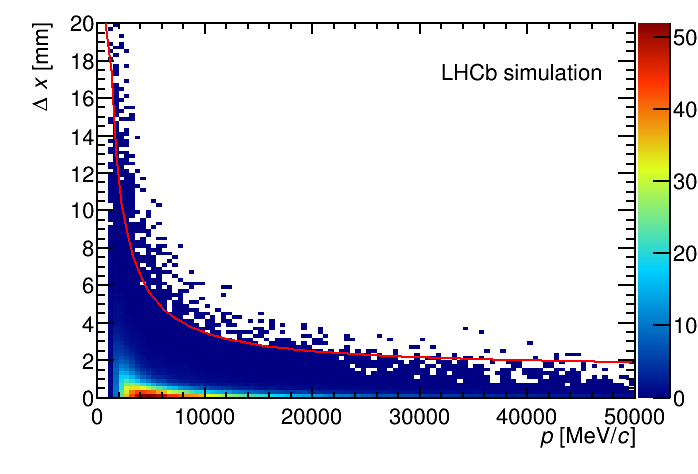
\includegraphics[width=0.49\linewidth]{figures/matchingDist1.png}
  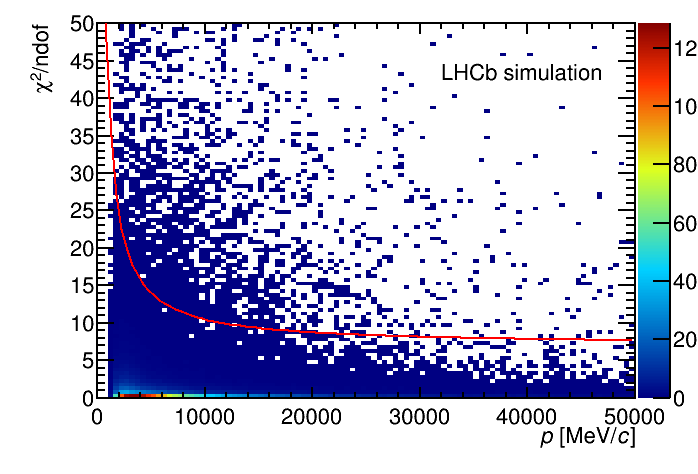
\includegraphics[width=0.49\linewidth]{figures/xChi2Cut1.png}
   \caption{Left: Distance between extrapolated track with one $x$ hit and
   (truth-matched) hit in the other $x$ layer. The red line represents the cut
   on the distance. Right: $\chi^{2}$ values for a fit to the $x$ hits
   (truth-matched), with the cut represented as a red line.
     \label{fig:matchingDist}}
 \end{center}
\end{figure}


A \chisqndf fit to the $x$ coordinate is then performed for each possible candidate, consisting
of the first hit in the $x$ layer, and one of the matching hits in the other $x$
layer. The magnet point is used as a further point to add enough degrees of
freedom for the fit. All track candidates are then sorted according to their
\chisqndf value, and track candidates are discarded if the \chisqndf value is
above:

\begin{equation}
\chi^{2}/\text{ndf}_{\text{max, x hits}} =  \texttt{FitXProjChi2Const} / p + \texttt{FitXProjChi2Offset}.
\end{equation}
If no hit could be found in the other $x$ layer, the track candidate is not rejected. 
It is kept without fit to search for hits in the $u$ layer. This allows for hit inefficiencies in the TT.

Due to the large combinatorial background, there can be many ghosts in this selection.
Tracklets with only two $x$ hits are prone to be ghost tracks, and it is
possible that the true combination of hits does not have the smallest \chisqndf.
Therefore, in the next steps, the first \texttt{MaxXTracks} tracklets are
considered whose \chisqndf value is within the range
(\texttt{MaxChi2DistXTracks}) to the lowest \chisqndf value.

\subsection[Search for hits in the $u$ layer]{Search for hits in the {\boldmath$u$} layer}
As the parameters of a track with (mostly) two hits are reasonably well
constrained, the search window in the $u$ layer can be smaller than 
those in the $x$ layers. Hits are searched around the track extrapolated to the
$u$ layer, where the $x$ position of the hit is updated by using the
extrapolated $y$ position. All hits within a search window are
considered, where the window size is defined as

\begin{equation}
\label{eq:uTol}
\Delta x =  \texttt{TolUConst} / p + \texttt{TolUOffset}.
\end{equation}
The parameters \texttt{TolUConst} and \texttt{TolUOffset} are determined
from simulation, illustrated in the left hand plot of Fig.~\ref{fig:uvLayerDist}.
The hits inside the window are then sorted according to their distance between the
extrapolation of the track and their actual position. For each hit which passes
this tolerance, a new tracklet is formed, until the maximum number of $xu$
tracks (\texttt{MaxXUTracks}) is reached. Each of these tracklets is then fitted
with a $\chi^{2}$ fit to obtain the best parameters for the following search in
the $v$ layer.


\subsection[Search for hits in the $v$ layer]{Search for hits in the {\boldmath$v$} layer}
As a last step in the hit search, hits in the $v$ layer are searched for. If the
track candidate already has 3 hits, a momentum dependent window is created
according to

\begin{equation}
\Delta x =  \texttt{TolVConst} / p + \texttt{TolVOffset}.
\end{equation}
See Fig.~\ref{fig:uvLayerDist} (right) for an illustration. In case the track only contains 2 hits,
Eq.~\ref{eq:uTol} is used to determine the size of the search window.
The hit that is closest to the extrapolation is added.


\begin{figure}[!htbp]
 \begin{center}
  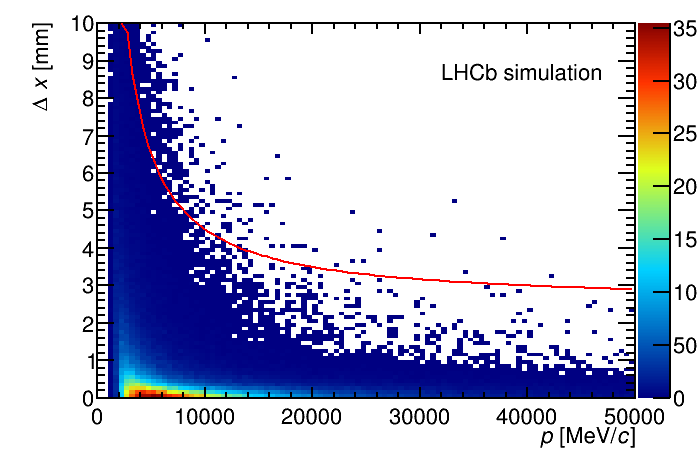
\includegraphics[width=0.49\linewidth]{figures/deltaXULayerCut1.png}
  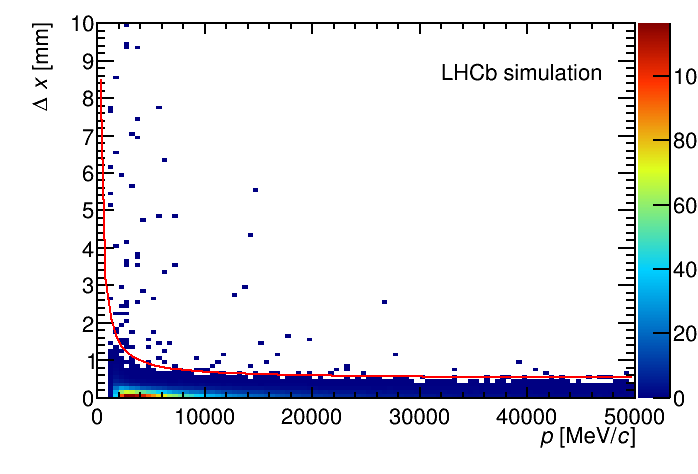
\includegraphics[width=0.49\linewidth]{figures/deltaXVLayerCut1.png}
   \caption{Left: Distance between extrapolated $x$-hits track and
   (truth-matched) hit in $u$ layer. The red line represents the cut on the
   distance. Right: Distance between extrapolated $xu$-hits track and
   (truth-matched) hit in $v$ layer. The red line represents the cut on the distance.
     \label{fig:uvLayerDist}}
 \end{center}
\end{figure}

\subsection[Calculation of $\chi^{2}$ and outlier removal]{Calculation of {\boldmath$\chi^{2}$} and outlier removal}
\label{sec:chi2}
At this stage, all possible hits in TT were added to the track candidates
(see Sect.~\ref{sec:addOverlap} for adding hits in the overlap region of TT), 
and a $\chi^{2}$ fit is performed. If the fit \chisqndf is smaller than a given value (\texttt{MaxChi2} and \texttt{MaxChi2ThreeHits} for candidates with 4 and 3 hits, respectively), 
the candidate is accepted and passed on to the next stage, otherwise the hit 
that contributes most to the $\chi^{2}$ is removed and the fit is repeated. 
The procedure is repeated until either the \chisqndf  is small enough, 
or there are hits in less than 3 planes left.
Furthermore, for each iteration of the fit, an explicit check is made
that each hit is still compatible with the estimated $y$ position of the track.

The $\chi^{2}$ fit only fits in 1 dimension by converting the displacement in
$y$ in a displacement in $x$.
The $\chi^{2}$ is therefore defined as:

\begin{equation}
\chi^{2} = \sum_{i \in hits} \frac{ \left(x_{i} - (x_{0} + t_{x}\cdot(z-z_{mag}) + c \cdot (z - z_{TT})(z - z_{TT}) + \left( \frac{dx}{dy} \right)_{i} y_{0}) \right)^{2}  }{\sigma_{i}^{2}}
\end{equation}
with $\left( \frac{dx}{dy} \right)_{i}$ the slope of the stereo plane and
$y_{0}$ the displacement in $y$. Note that $c$ is fixed, see Sect.~\ref{sec:trackModelTT}.
Forming partial derivates with respect to $x_{0}, t_{x}$ and $y_{0}$, a set of
linear equations can be solved to obtain the three free parameters. For details
of this calculation, see for example Ref.~\cite{Stahl:DiplomaThesis}.

\begin{figure}[!htbp]
 \begin{center}
  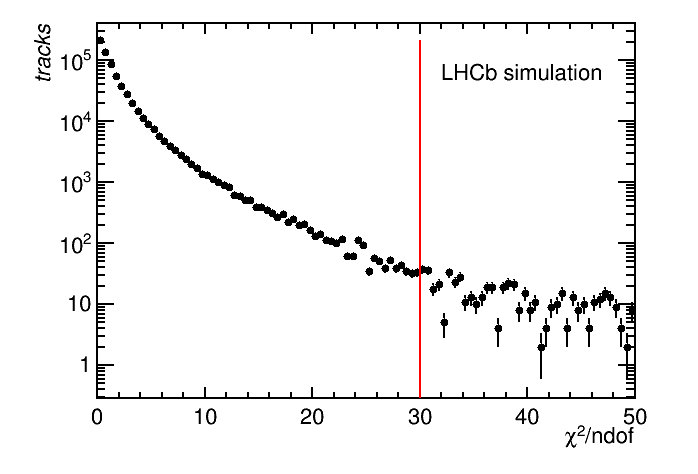
\includegraphics[width=0.49\linewidth]{figures/chi2Cut1.png}
  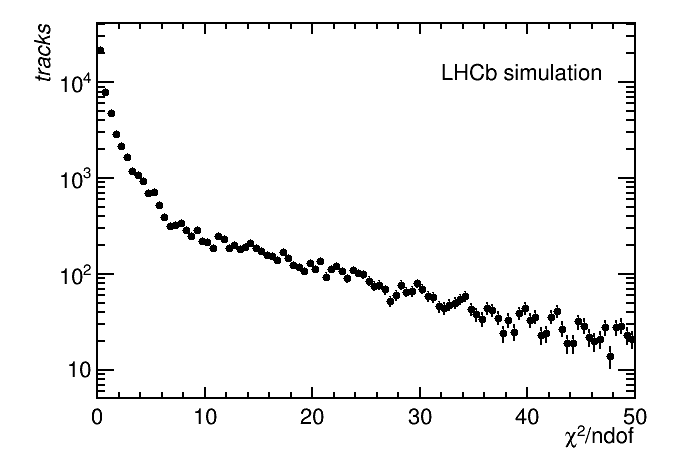
\includegraphics[width=0.49\linewidth]{figures/chi2Cut3Hits1.png}
   \caption{Left: $\chi^{2}$ distribution for truth-matched tracks with 4 or more
   hits. The maximum allowed value is 30. Right: $\chi^{2}$ distribution for
   truth-matched tracks with 3 hits. The maximum allowed value is 50.
   \label{fig:chi2Cuts}}
 \end{center}
\end{figure}

\subsection{Accepting the candidates}
\label{sec:acceptCandidate}
The track candidate is accepted in the final selection of track candidates,
if it fulfills the following criteria. All cut values were trained on simulated data, 
with the goal to keep a balance between signal retention and background rejection. 

\begin{itemize}
\item It has at least three hits in at least three different layers of the TT.
\item The \chisqndf is below a given threshold. This value is different for
three-hit tracks (\texttt{MaxChi2ThreeHits}) and tracks with four or more hits (\texttt{MaxChi2}),
see Fig.~\ref{fig:chi2Cuts}. 
\item It contains at least as many hits as any other candidate for a given T track.
\item The track has a pseudorapidity larger than 1.8 and smaller than 5.2.
\item At least \texttt{NMinHighThresHits} of the hits have the high-threshold
bit set.
\end{itemize}

The following checks are repeated, this time using the fit result instead of the initial estimates.

\begin{itemize}
\item The momentum estimate is compatible with the momentum estimate from the
T track.
\item The track has a minimum momentum \texttt{MinMomentum} and a minimum $p_{T}$ \texttt{MinPt}.
\item The track does not point into the beampipe.
\end{itemize}

\subsection{Addition of overlap hits}
\label{sec:addOverlap}
For all track candidates which are retained at this stage, hits in the overlap
regions of the TT detector are searched for. 
TT modules are staggered in the $z$ direction with an overlap, in order to cover the insensitive region of the modules and to not lose efficiency. A hit qualifies as an overlap hit if it
is within a certain distance to the extrapolated track (\texttt{OverlapTol}), in the same
layer as an already existing hit, but at a
different $z$ position.

As adding an additional hit will change the properties of the track, the track
is again fitted with the potential removal of outliers. It is then again checked
that it fulfills the criteria in Sect.~\ref{sec:acceptCandidate}.


\section{Selection of T tracks }
\label{sec:TSeed}

T-seeds together with TT hits constitute an input to the LongLivedTrackign (LLT) algorithm and their quality has a direct and significant impact on the algorithm performance. Therefore, the very first and crucial step is a filtering procedure, which purpose is to increase purity of the set of T-tracks by rejecting as many unreconstructible track as possible. This also allows to reduce the execution time since the combinatoric is greatly reduced. A previous analysis showed that T-seed filtering based on a simple linear selection using track quality and kinematic variables is not feasible. Therefore, an idea of using Machine Learning techniques was proposed. This section is dedicated to present all studies, starting from preparing and understanding training dataset, to selecting the best model, to attempting to understand the model's prediction. 

This problem is similar to the email spam detector, in both cases it is desired to keep all true events and remove as much as possible false events. The nature of this problem reflects in selection of the cutoff probability threshold.  

\subsection{T-seed classifier: Data Collection} 

The very first step within the training Machine Learning model pipeline is a data collection. It is not possible to build any statistical model without collecting sufficient amount of data. From the perspective of this project the data was generated by the Monte Carlo simulation. To extract required data a dedicated tool within Brunel project was implemented. This tool is dedicated to match track with MC particle. The particle is considered as matched to a given track if they share at least 70\% of the hits. Such a link allows to assign a target value to tracks.    

One of the most difficult problem during the data preparation step was choosing the track labeling policy. Within this process, for each T-seed a target flag was assigned. What is crucial, every time when a strategy is changed, the entire process of model selection and training has to be redone, which happens at least three times during author's study. The final labelling strategy tells the track is consider as a reconstructable, later called a \textbf{true T-seed}, when it meets the following criteria:
\begin{itemize}
    \item Has to be associated with a valid Monte Carlo particle;
    \item From above association the electron is excluded; 
    \item Has at least two hit associated with TT station;
    \item no hits in the Velo detector. 
\end{itemize}

Those criteria can be justified by definition of the Downstream tracks, which are created by the particles that decays outside of the Velo detector. 

\section{T-seed classifier Exploratory Data Analysis}

The next step that were performed is Exploratory Data Analysis. This step is essential to understand the input data, find patterns, relationships, or anomalies that can influence the outcome of the model prediction.   

\begin{figure}
\centering
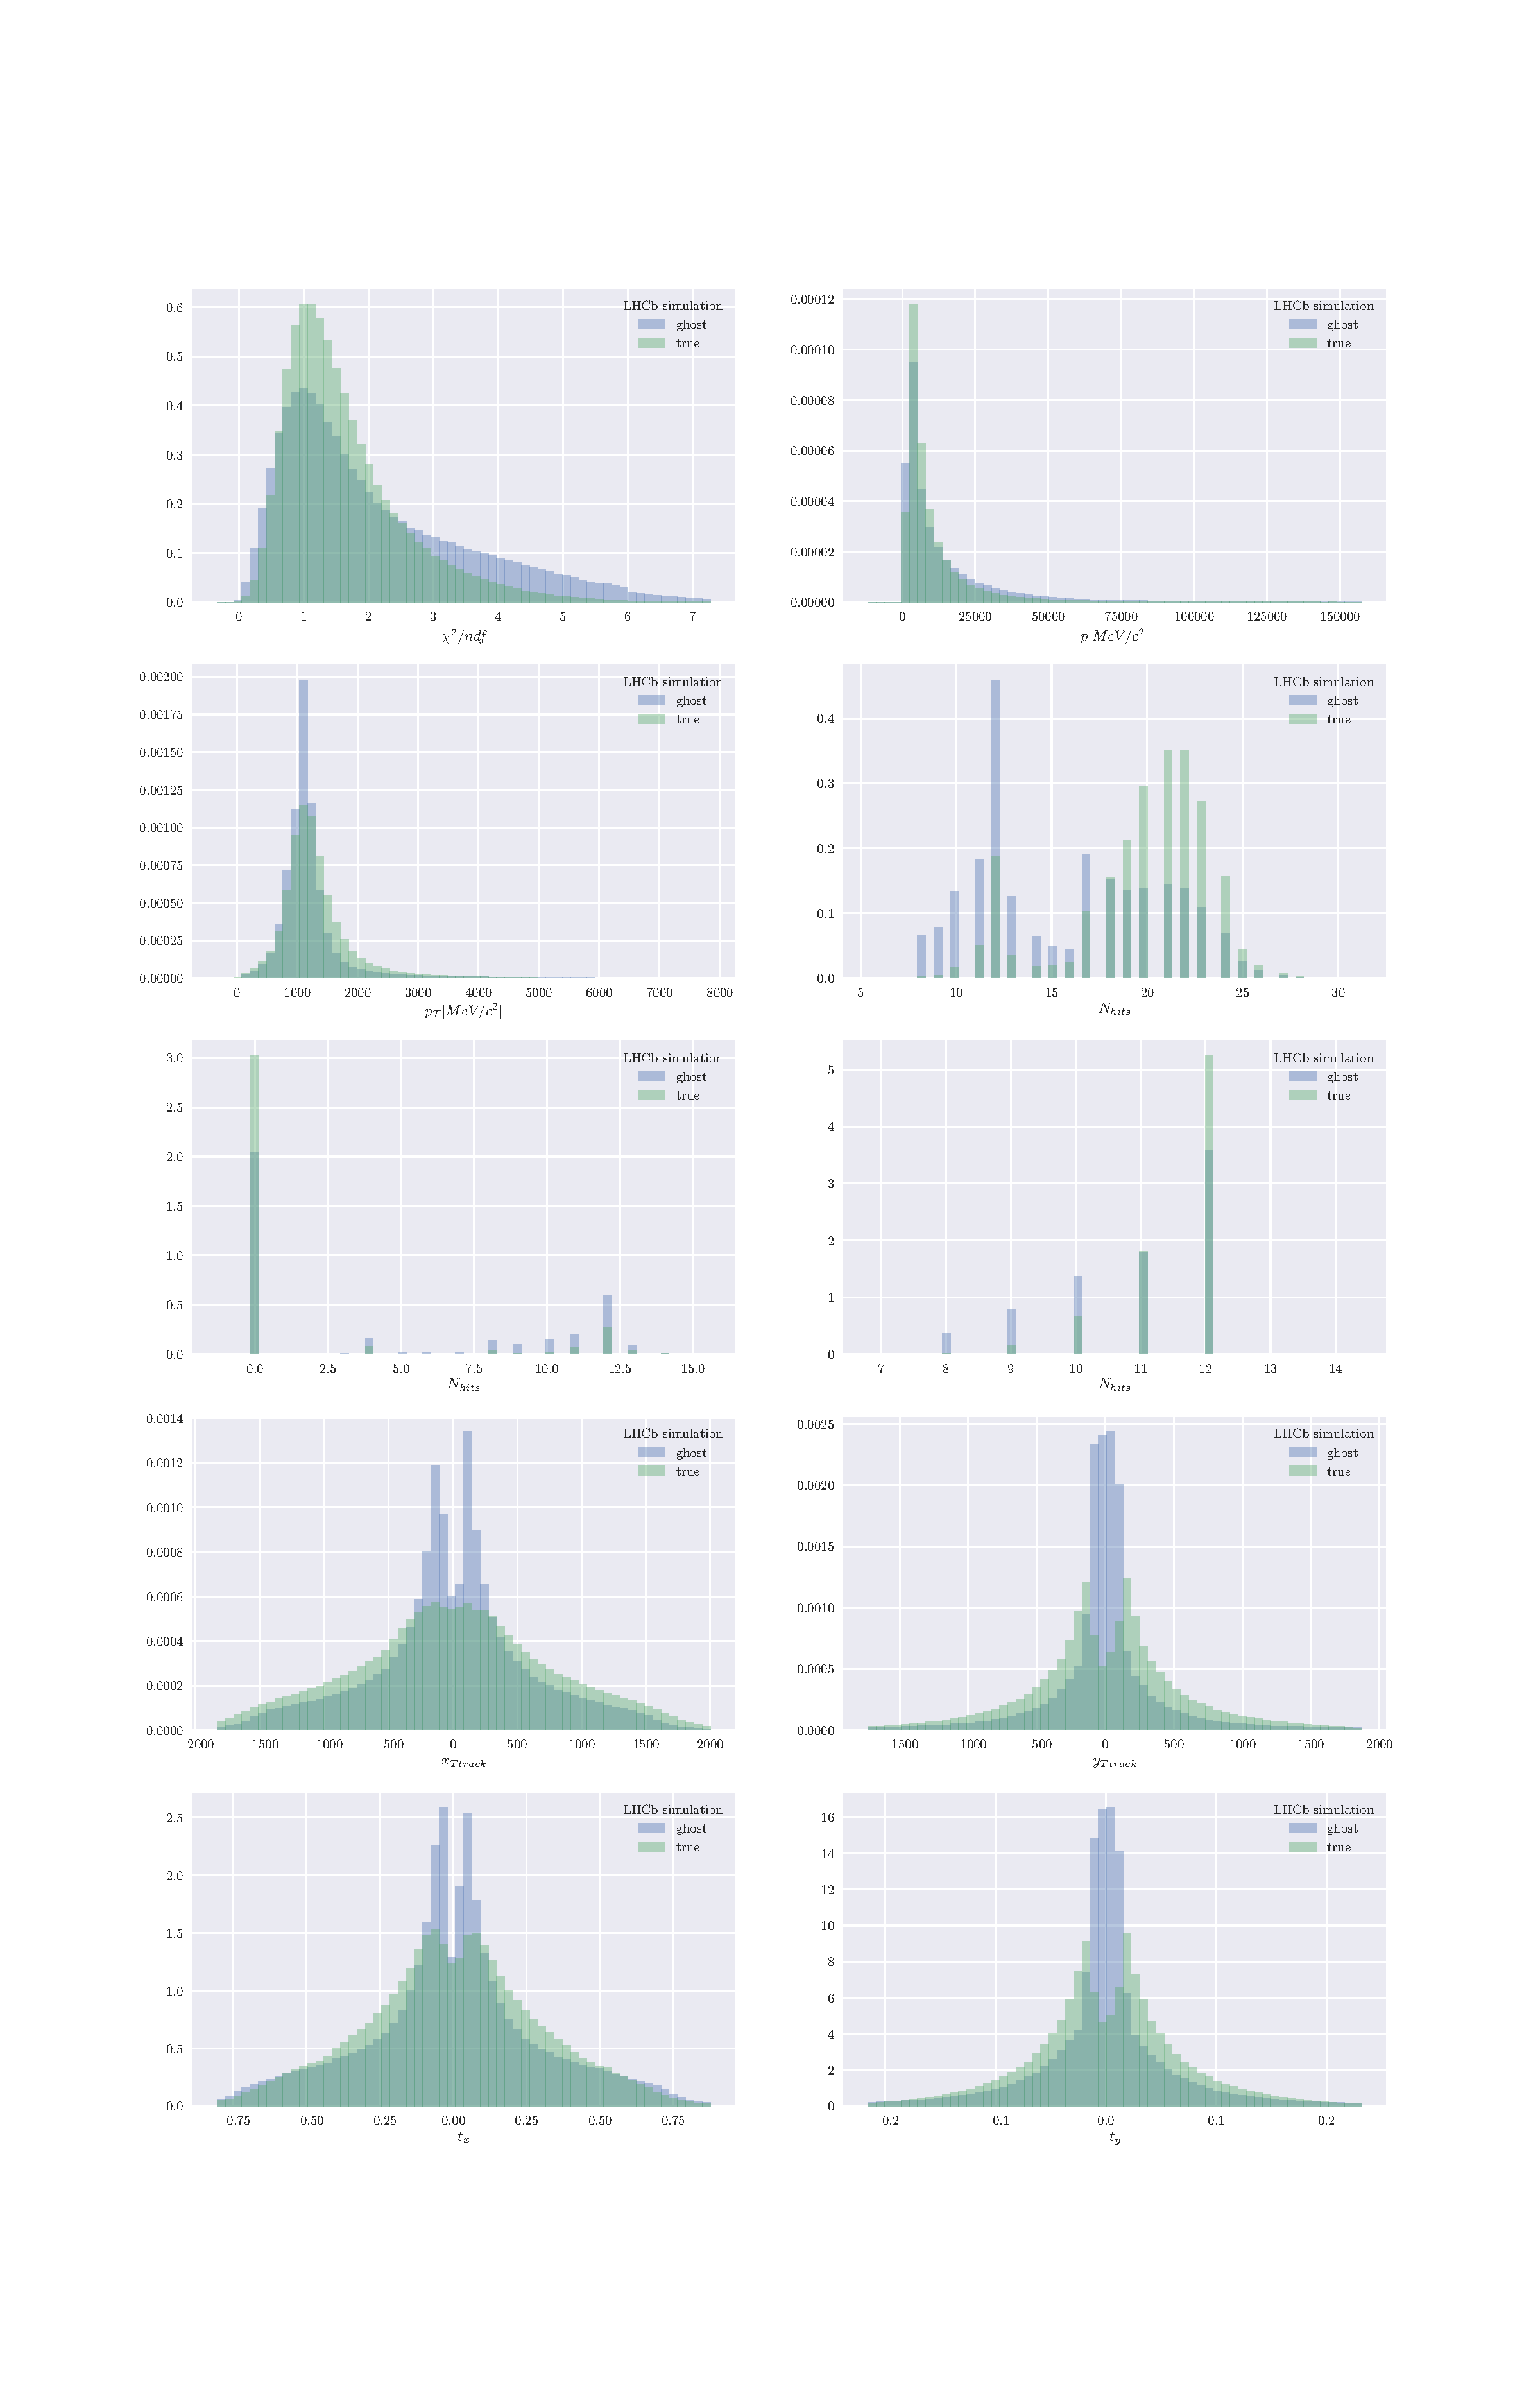
\includegraphics{figures/features.pdf}
\caption{Distribution of the input variables used to train T-Seed filter. The sample was extracted using a $B_0\rightarrow J/\psi K_S^0 $ samples decays. The green solid histogram is the signal distribution, while the light blue
distribution is the background.
\label{fig:input features}}
\end{figure}

The search for the best classifier was performed using a simulated data sample containing signal events $B^0\rightarrow J/\psi K_S^0 $ decays events. The entire dataset contains more than 2 million T-Seeds. TO avoid bias that could be introduced by considering only one magnet polarization the training dataset contains the data of both magnet polarities.  
The following variables were considered as an initial features set. Further input dimentionality enhancement was done in the feature engineering phase. 

\begin{itemize}
    \item $\chi^2/ndf$: T-track $\chi^2/ndf$ determined by the PatSeeding algorithm, which is defined in the following way: 
    \begin{equation}
        \chi^2 = \sum_{hits i} \frac{1}{\sigma_i^2} \left( \frac{x_i-x_{track}(z_i)}{\cos \alpha} \pm r_{drift} \right) 
    \end{equation}
    where: $(x_i, z_i)$ is the $x$ coordinates of the i-th hit at the $y(z_i)$ predicted form the track model, $\sigma_i$ is the hit postilion uncertainty and $r_{drift}$ is the drift radius for Outer Tracker hits or 0 for the Inner Tracker. 
    \item $p$: the absolute momentum of a T-track; 
    \item $p_t$: the transverse momentum;
    \item $N_{hits}$: number of hits constructing tho a given T-seed;
    \item $x_{T track}$: the $x$ position of the T track's first state; 
    \item $y_{T track}$: the $y$ position of the T track's first state;
    \item $t_x$: the slope of the track in the $x-z$ plane;
    \item $t_y$: the slope of the track in the $y-z$ plane;
    \item $r_{track}$: the distance from the beam line, z-axis, calculated for the first state. The $r_{track}$ is calculated as follow:
    \begin{equation}
        r_{track} = \sqrt{x_{T track}^2 + y_{T track}^2}
    \end{equation}
    \item $\eta$: pseudorapidity. 
\end{itemize}
Each of above feature distributions is presented in the figure \ref{fig:input features}. It is clearly visible that the data is not linearly separable and the distribution for both true and false classes are very similar to each other. 

One of the most popular way to show the dependencies among features is to calculate  the Pearson correlation coefficient $\rho$. The formula for $\rho$ is:

\begin{equation}
    \rho(X,Y) = \frac{\mathbb{E}(X-\mu_x)(Y-\mu_y)}{\sigma_x \sigma_y}
\end{equation}

This parameter has value in the range of $<-1,1>$. The value of 0 indicates no correlation, the -1 and 1 implies strong negative and positive correlation respectively. In order to visualize all of the correlation coefficients, so called correlation matrix was created. Figure \ref{fig:corrMatrix} shows two correlation matrices, the data separation was done according to the target flag. There is no significant difference between true and false T-Seeds correlation matrices. This gives the first impression, that the classification task is hard. 

\begin{figure}
  \centering
  \begin{tabular}{@{}c@{}}
    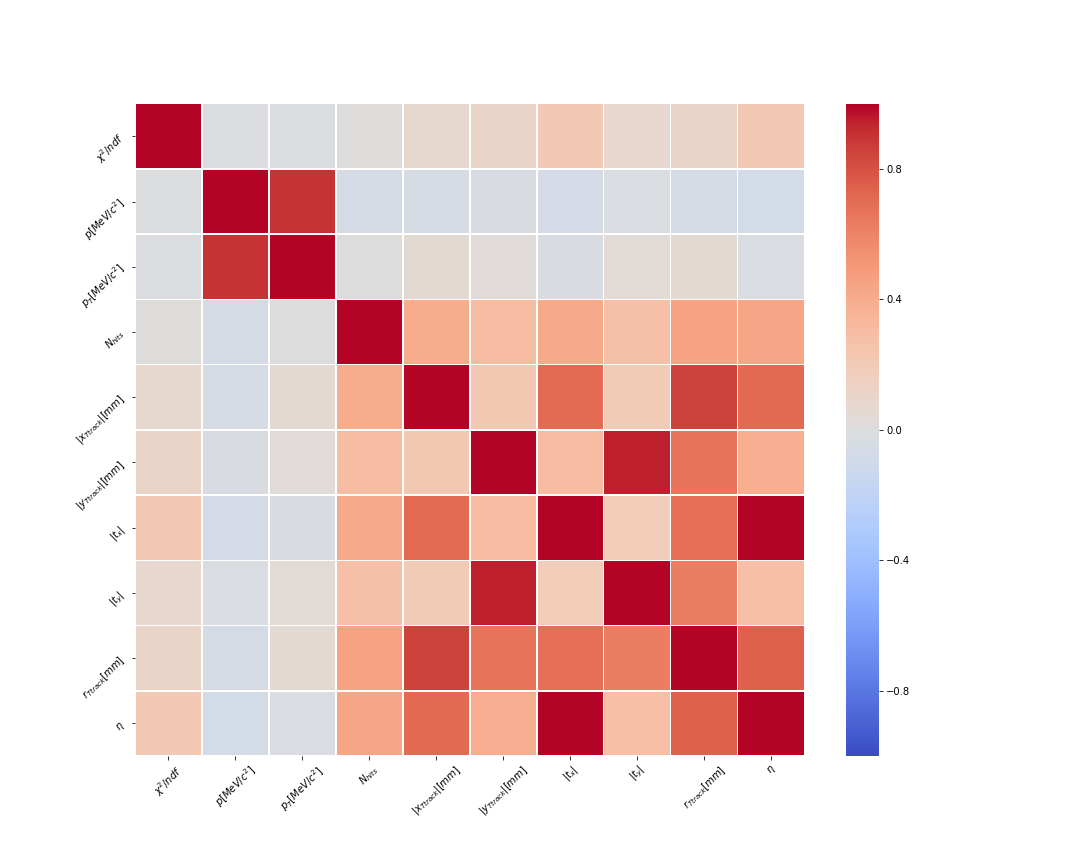
\includegraphics[width=\linewidth]{figures/corr_matrixTrue.png}
  \end{tabular}

  \vspace{\floatsep}

  \begin{tabular}{@{}c@{}}
    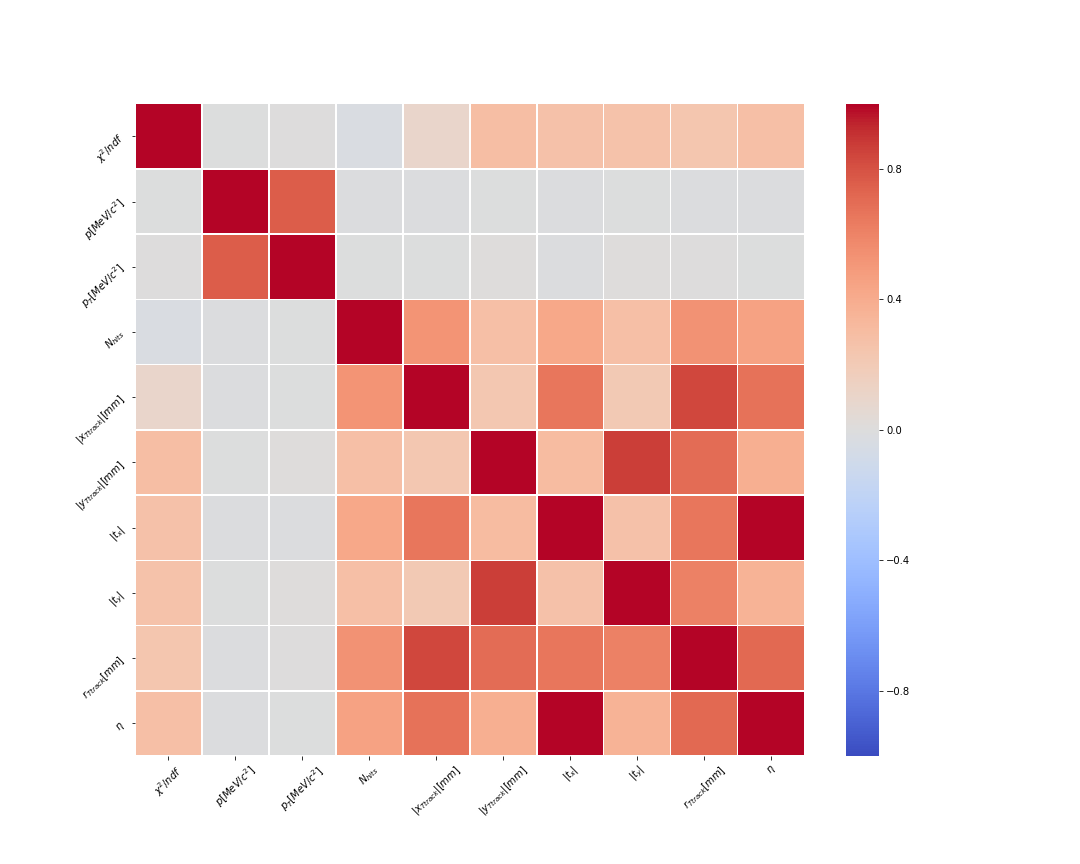
\includegraphics[width=\linewidth]{figures/corr_matrixFalse.png}
  \end{tabular}

  \caption{Pearson  correlation matrix that were obtained using a subset of input features. The top plot shows correlation matrix for True T-seeds. The bottom plot presents similar Pearson correlation matrix generated using the ghost T-Seeds.  
\label{fig:corrMatrix}}  
\end{figure}

    
The Pearson  correlation coefficient is a good metric to detect linear dependencies among features, but it is not sensitive to more sophisticated relations. To overcome this limitation the pair-plot was made, showed in figure \ref{fig:Pair plot}. A pairs plot allows to see both distribution of single variables and relationships between two variables, which is carried as a scatter plot. This is particularly interesting to visually inspect how the variables are distributed for a given pair of attributes. To make this plot more readable the data were split into two groups according to the target flag. That kind of plot allows to make an initial guess on the features importance. 

\begin{figure}[!h]
\centering
\hspace*{-2cm}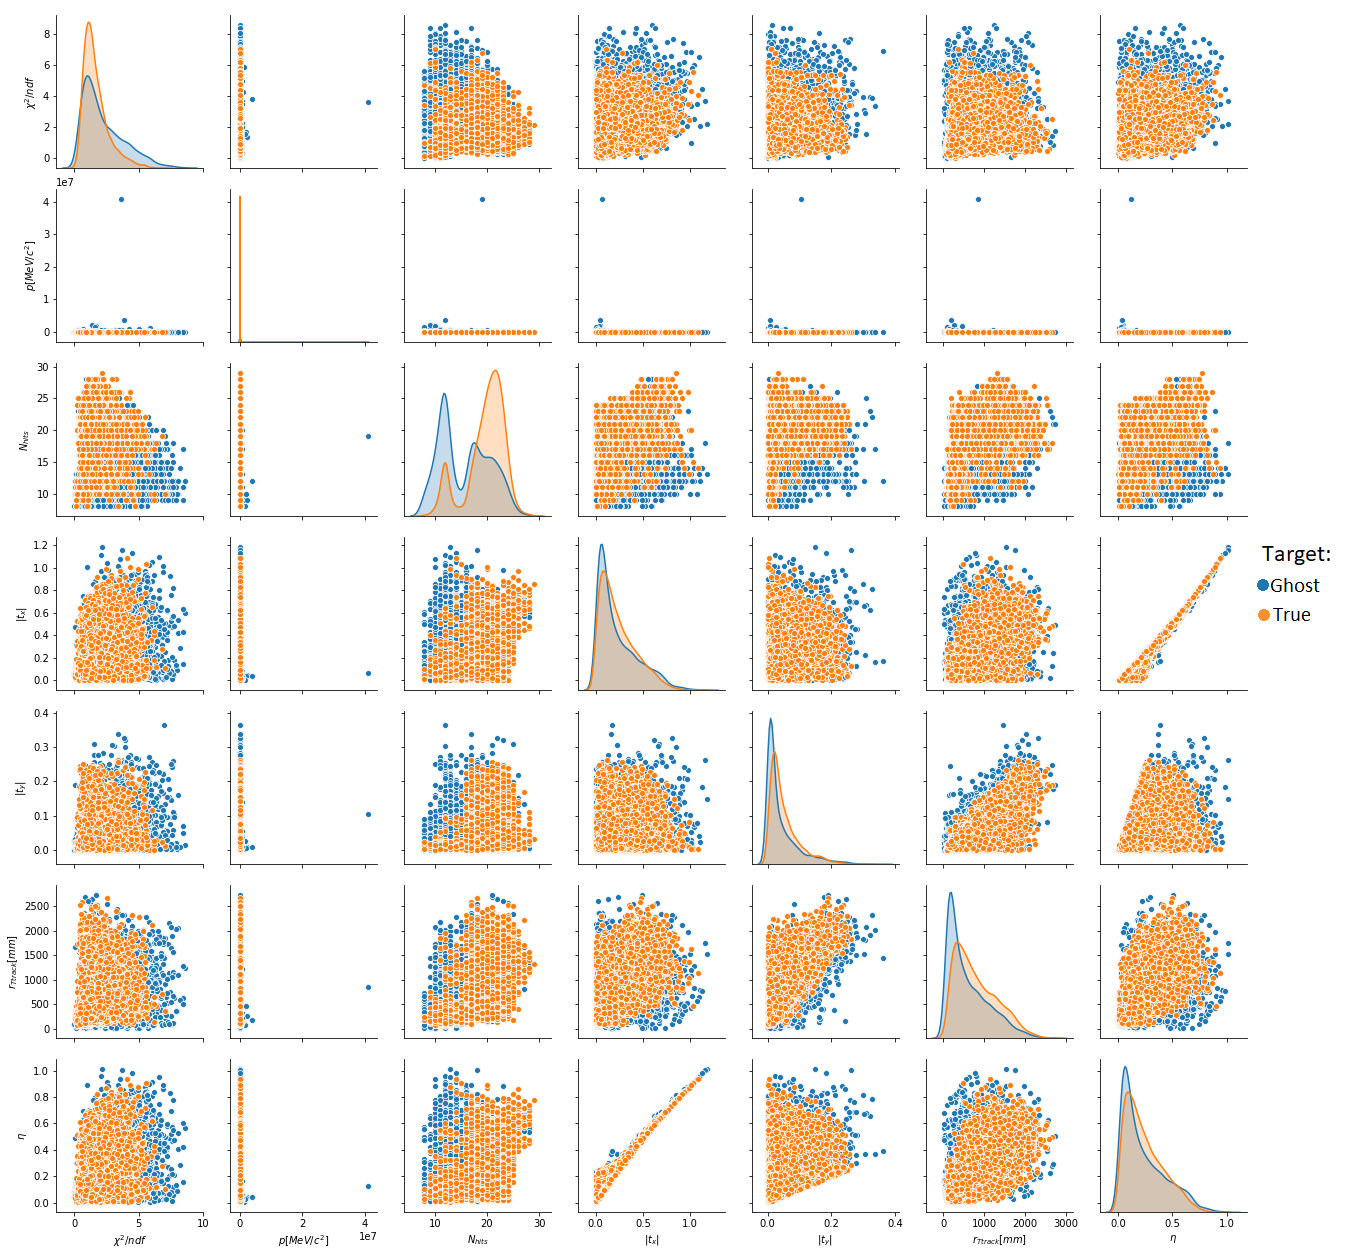
\includegraphics[width=1.3\textwidth]{figures/pair_plot.png}
\caption{Pair-plots that were generated using subset of input features. The input data was separated based on the value of the target flag. The blue points represents ghost T-Seeds and the orange points represents true T-Seeds. }
\label{fig:Pair plot}
\end{figure}

\section{T-Seed classifier: baseline}

This section dedicated to present the Machine learning study baseline, which was implemented as training of two models, kNN and logistic regression.
 
These two models were selected as a baseline due to their simplicity and a short amount of time that is required to train them. The simplicity, except for the model's underlying idea, is manifested by a small number of hyperparameters that needs to be tuned. The baseline score is the entry point to the Machine Learning study. This score  should be over-performed by all of the more sophisticated models. It also provides an initial understanding of how hard the classification problem is. In some cases, excluding this one, the baseline could be an average human performance on the task. 

\subsection{$k$NN} 
\label{sec:KNN_result}

The $k$NN described in section \ref{sec:knn}, is a model that has two hyperparameters that need to be selected - a number of neighbors and the distance metric. The training pipeline contains of the following steps:

\begin{itemize}
    \item Data extraction;
    \item Data normalization: each of the features were normalized by removing the mean and scaled to unit variance. Centering and scaling happen independently on each feature by computing the relevant statistics on the samples in the training set. 
\end{itemize}
The mentioned pipeline were implemented using sklearn framework\cite{sklearn}.  

Figure \ref{fig:kNN score} presents the ROC AUC score versus the number of neighbors. The score and its uncertainty were obtained using the cross-validation method. The classifier's score maximum value, ROC auc score 76, were obtained for $k \approx 210$.  

\begin{figure}[!h]
\centering
\hspace*{-1cm}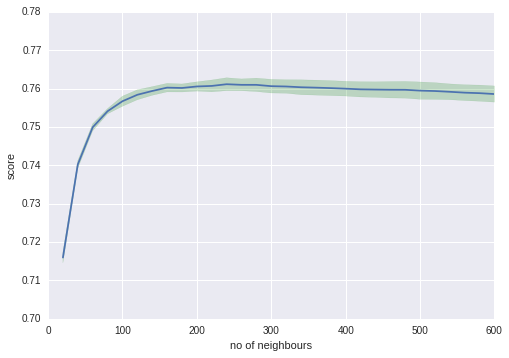
\includegraphics{figures/knn.png}
\caption{The kNN performance plot, ROC auc score vs the number of neighbor. The green shaded area represents score's one standard deviation region.}
\label{fig:kNN score}
\end{figure}

\subsection{Logistic Regression}

The second baseline mode is Logistic Regression described in section \ref{sec:LogReg}, and implemented using sklearn framework.
The input to this model has to be normalized, which is the only preprocessing step that was applied, therfore the data processing pipeline was identical to the one described in section \ref{sec:KNN_result}. 
To maximize the classifier score analysis of the L1 and L2 regularization constants were conducted. These two hyperparameters were introduced to reduce overfitting, although as presented in figure \ref{fig:RL_L1} none of them has significant impact on the classifier performance.


\begin{figure}[h]
  \centering
\begin{tabular}{c c}
\subfloat{{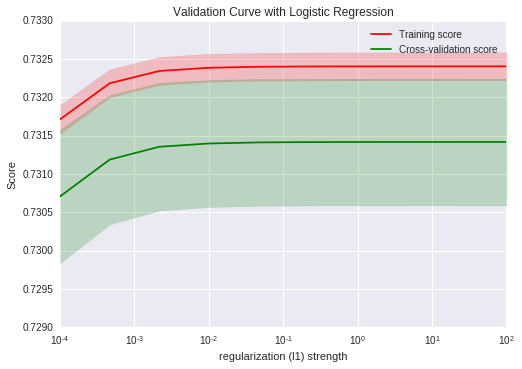
\includegraphics[width=0.5\textwidth]{figures/RL_L1.png} }}%
    \subfloat{{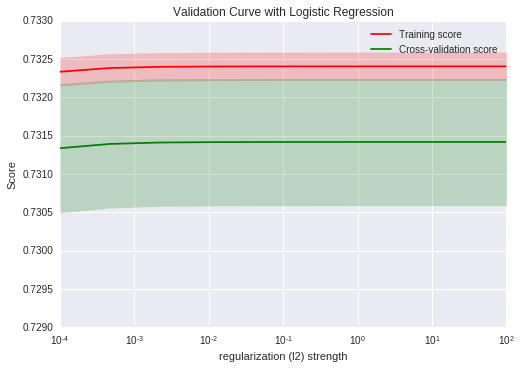
\includegraphics[width=0.55\textwidth]{figures/RL_L2.png} }}%
\\
\end{tabular}
   \caption{Logistic Regression validation curves. The plots present the impact of L1 (left) and L2 (right) regularization on classifier performance.  
\label{fig:RL_L1}}  
\end{figure}

  
Finally, to check the stability of the prediction, the study of model performance versus a number of training entries was performed. The results are shown in figure \ref{fig:LR_NE}. This plot indicates the biggest limitation of the linear model. The model’s performance is not affected by increasing the amount of data, that were used to train them.  

\begin{figure}[!h]
\centering
\hspace*{-1cm}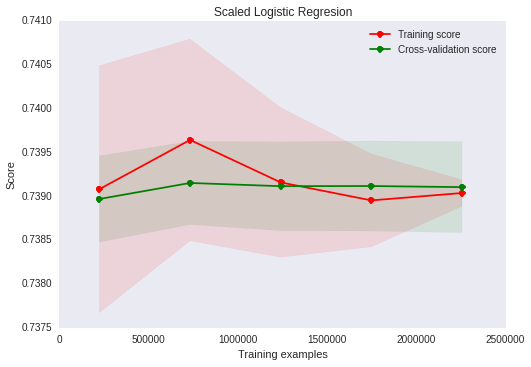
\includegraphics{figures/LogReg_te.png}
\caption{The Logistic Regression model performance vs. the number of training examples}
\label{fig:LR_NE}
\end{figure}

The score, measure as ROC AUC, obtained by the Linear Regression model is about 74\%, which is slightly worst than the result obtained by the kNN classifier.  

\section{T-Seed classifier: study based on XGBoost model}

The previous two models were selected to provide the baseline scores. This section presents the training strategy and results that were obtained using the XGBoost model. 

The first step within this analysis was to train the model with default values of hyper-parameters to get a better understanding of the model initial performance. This step was also executed to estimate the number, or at least the order of magnitude, of weak learners that need to be added to the boosting model. This number can be estimate by detecting moment when model performance starts to saturate. 

The model saturation is a situation when adding a new tree has no positive impact on the performance, measured on both training and the validation datasets. This effect can be easily detected using a learning curve plot. The learning curve plot is a two-dimensional plot with classifier performance on the y-axis and a number of trees on the x-axis. The saturation effect occurs when learning curve Plateau. 

The initial training allows estimates of the number of trees to be around 700. The other hyperparameters, that were taken into consideration are listed below:

\begin{itemize}
    \item \textbf{learning rate} - shrinkage parameters (see section \ref{sec:xgboost}), which control the weight of new tree added to the model;    
    \item \textbf{max depth} - a maximum allowed depth of each of the trees, increasing its value makes week learners more complex and more likely to overfit. 
    \item \textbf{gamma} - minimum loss reduction required to make a further partition on a leaf node of the tree. Increasing the gamma values makes the boosting process more conservative. 
    \item \textbf{min child weight} - a minimum sum of instance weight needed in a child to make a split. If the tree partition procedure step produces a leaf node with a sum of instance weight smaller than \textbf{min child weight}, then the building tree process is terminated. This parameter can be interpreted as a minimum number of instances needed to be in each node.
    \item \textbf{colsample by tree} - subsample ratio of features used to construct a particular tree. Subsampling occurs once for each tree. 
    \item \textbf{reg alpha, reg lambda} - regularization factor L1 and L2 on weights.      
    
\end{itemize}

Taking into consideration the dimensionality of this optimization problem, as well as the fact that each training iteration takes about 1 hour the Bayesian Optimization seemed to be the most promising approach to tune the hyperparameters. Although, all three hyperparameters tuning strategies described in section \ref{sec:hyperparameters} were applied. Figure \ref{fig:hyperparameter_xgboost} presents the Bayesian optimization results in a form of coverage plot, where each of the scores is a ROC AUC score calculate using three-fold cross-validation method. Within the presented experiment the Gaussian process was selected as a surrogate function and Expected Improvement played the role of an acquisition function. Each training round was terminated once the performance on the test dataset has not improved after a fixed number of training iterations. This method is called early stopping, and its main purpose is to prevent training the model when it performance saturates. The positive site effect of this method is reduction of overfitting. 

The Bayesian optimization needs about 40 iterations to find the optimal hyperparameter set \footnote{In this context \textbf{optimal} is consider to be the best one for a given subset of hyperparameter's ranges, it is not guaranteed to be globally optimal}. The Grid and Random Search provide similar results, although each of these methods requires more optimization steps to find a set that works as good as the one produced by Gaussian optimization. 

\begin{figure}
\centering
\hspace*{-1cm}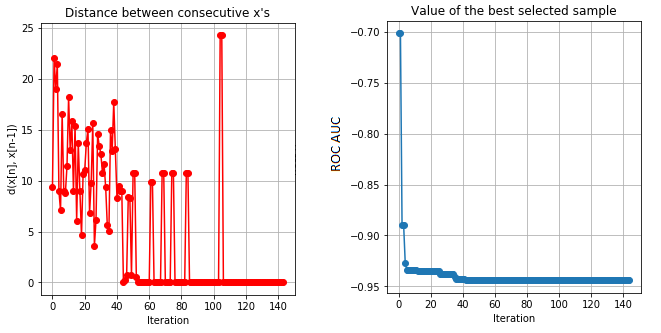
\includegraphics{figures/GaussianOptXgboost.png}
\caption{Bayesian optimization coverage plots. The left plot presents iterations vs. distance between consecutive selected hyperparameters sets, the right plot shows iterations vs. the ROC auc score of the current model.}
\label{fig:hyperparameter_xgboost}
\end{figure}

Using selected by the Bayesian optimization method set of hyperparameters, the final xgboost based model achieved a score, measured as an area under the ROC curve of 94\%. The figure \ref{fig:xgboost trainig} presents three different learning curve plots. The first one shows the training progress measured as a reduction of the cross-entropy loss versus the number of trees constituted the model. The second one presents the binary classification error rate, which is calculated as a ratio between a number of wrongly classified cases to all test cases, vs the number of training iterations. The final one presents how the area under the ROC curve versus number of weak learners. The learning curve plots were obtained using a test sample that constitutes 20\% of the entire dataset. 


\begin{figure}
\centering
\hspace*{-1cm}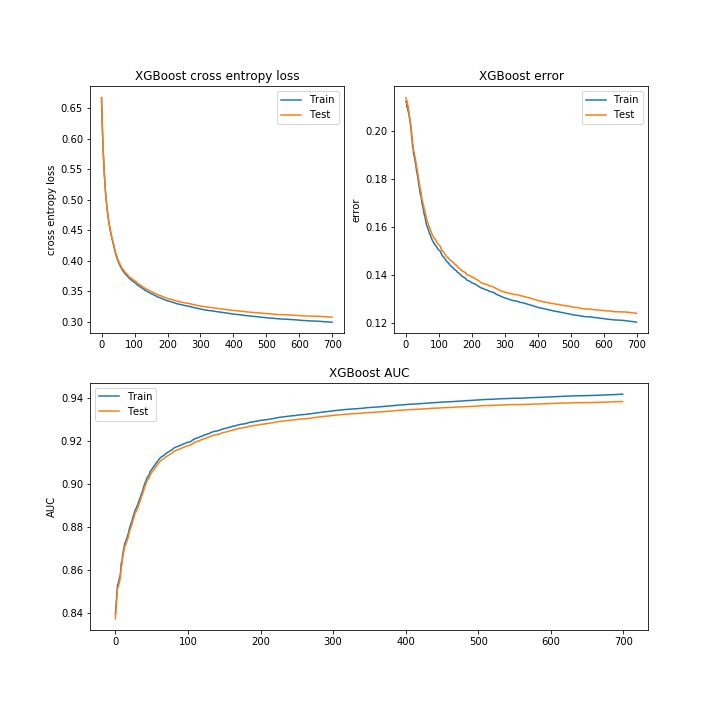
\includegraphics{figures/learning_curve_xgboost.png}
\caption{Learning curve for the XGBoost classifier. The upper left plot presents cross-entropy loss function vs. a number of week estimators, the right upper plot shows miss classification vs the number of trees. The bottom plot presents how the ROC AUC versus training iterations.}
\label{fig:xgboost trainig}
\end{figure}


The learning curve plot is one of the most important tool to visually investigate whether model is overfitted.  
Overfitting refers to a model that has learned the training dataset too well, including the statistical noise or random fluctuations in the training dataset. This effect becomes apparent when the performance gap between training and validation curves increase when increasing the model complexity, which is shown in figure \ref{fig:xgboost_overfitting} .Figure \ref{fig:xgboost trainig} clearly indicates that the model perform very well and the effect of overtraining is not present \footnote{This conclusion is based on a specific testset, that constitutes examples comming from the same distribution.}. 


\begin{figure}
\centering
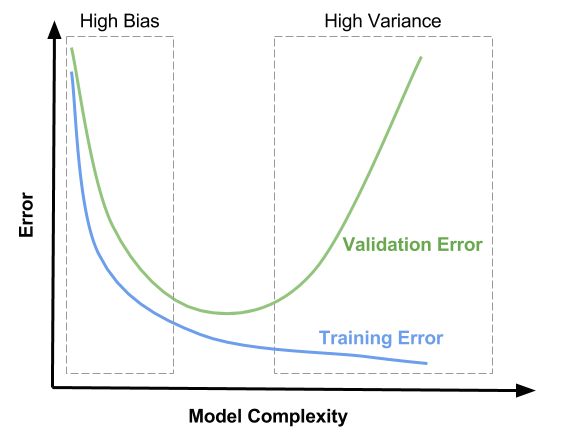
\includegraphics[scale=0.6]{figures/bbdt_overfitting.png}
\caption{Cartoon presenting different behaviour of the Boosted Decision Tree classifier. The leftmost region represents the model that is undertrained which is reflected in decreasing learning curves. The rightmost region corresponds to the model that is overtrained, in such a case validation curve is increasing while train curve is decreasing. }
\label{fig:xgboost_overfitting}
\end{figure}



\section{T-Seed classifier as a bonsai Boosted Decision Tree }

As described in section \ref{sec:bbdt}, the evaluation of the continuous complex classifier is too expensive (from the perspective of CPU time) to deploy that kind of model within HLT2. Therefore, the model was binarized and deployed in the form of bBDT, which is visualized in figure \ref{fig:bbt_structure}. 



\begin{figure}[h]
\centering
\hspace*{-1cm}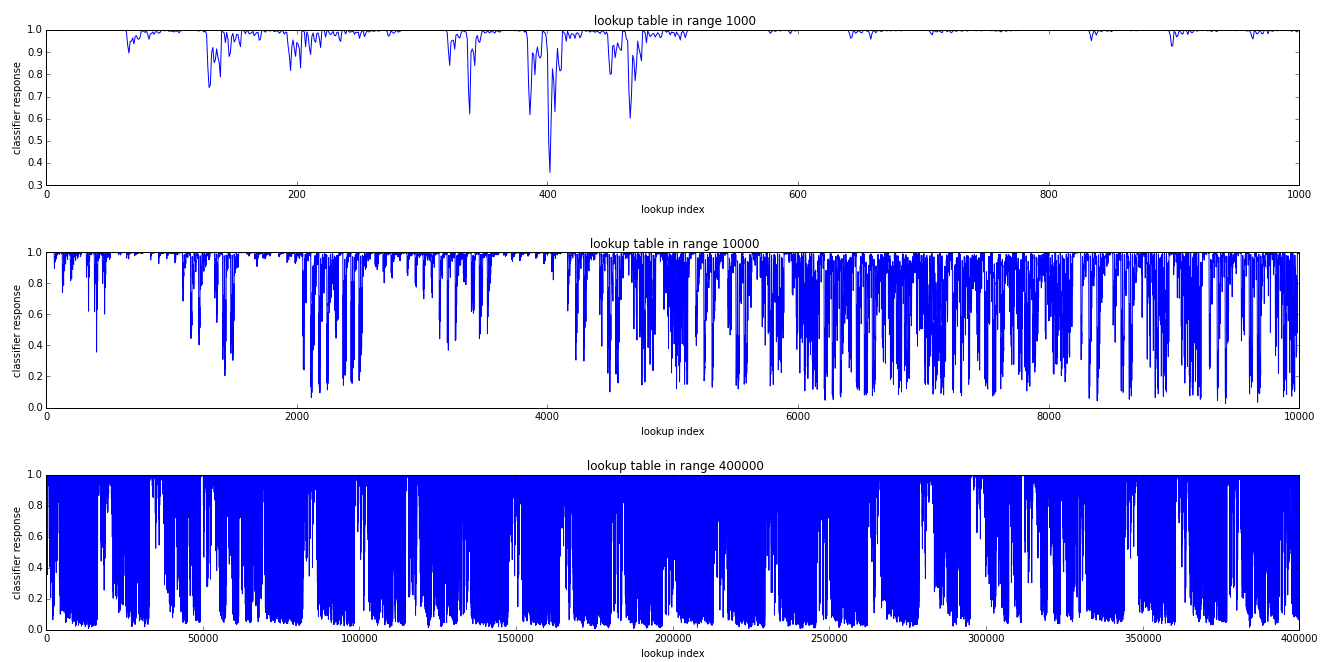
\includegraphics{figures/BBDT_lookup.png}
\caption{Structure of the bBDT lookup table. Each of the plot presents different range of lookup tables (x-axies) versus reposnse of the classiers (y-axies).}
\label{fig:bbt_structure}
\end{figure}



The response of the binned BDT and its ROC curve are presented in figures  \ref{bbdt response} and \ref{fig:ROC binned} respectively. A slight drop in the performance of the binned classifier with respect to the full one has been noted. The figures of merit measured for the bBDT algorithm amounted to 87\%. Based on the ROC curve the classification threshold was selected to be $0.07$, see section \ref{sec:CUT finetuning} for more details. This highly conservative value of the threshold was advocated by the fact that the final classifier has to keep more than 99\% of the true seeds. Nevertheless, this threshold value allowed to remove 30 \% of the fake seeds, thus significantly decrease the ghost rate, formally defined in section \ref{sec:physic_performance}.   



\begin{figure}
\centering
\hspace*{-1cm}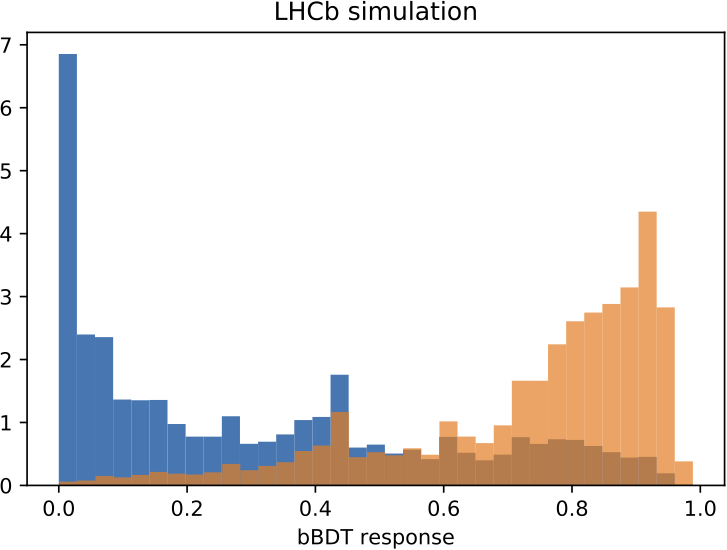
\includegraphics[scale=0.6]{figures/bbdt_response.png}
\caption{bBDT classifier output distribution, blue is background and orange is signal }
\label{fig:bbdt response}
\end{figure}


\begin{figure}
\centering
\hspace*{-1cm}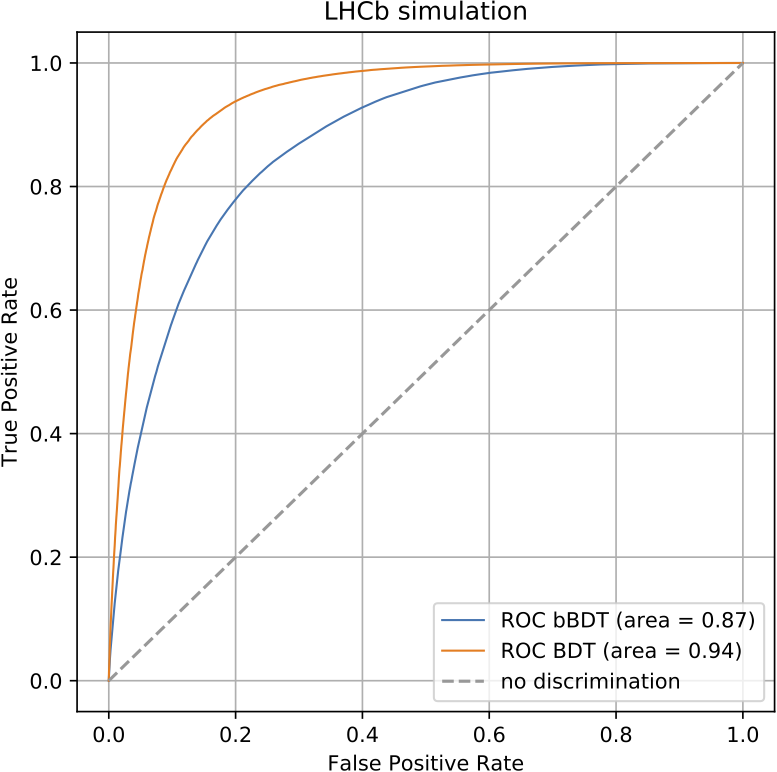
\includegraphics[scale=0.6]{figures/bBDT_roc.png}
\caption{Comparison of ROC curves for selecting true T tracks using a simulated $B_0\rightarrow J/\psi K_S^0 $ sample before and after binning.}
\label{fig:ROC binned}
\end{figure}





\begin{figure}
\centering
\hspace*{-1cm}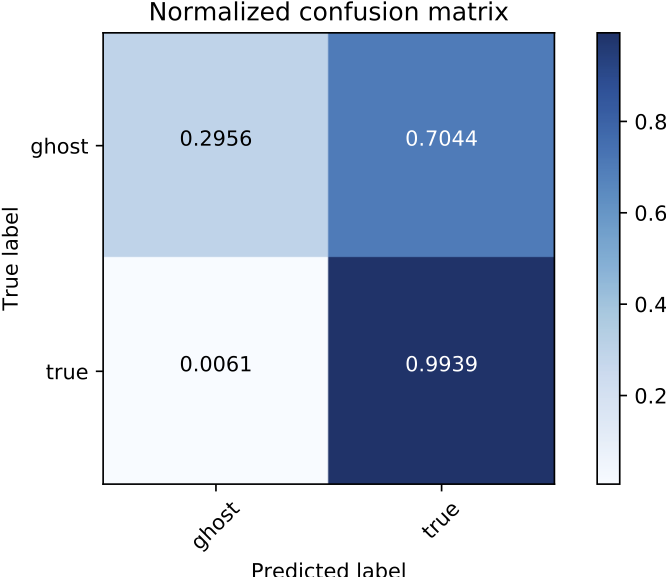
\includegraphics[scale=0.6]{figures/bBDT_normalized_cm.png}
\caption{Normalised confusion matrix determined for the trained bonsai BDT (binned) model.}
\label{fig:CM normalized}
\end{figure}



\section{T-Seed classifier: model output interpretation}

This section is dedicated to emphasizing the importance of the model's interpretability. As presented before the T-Seed filter achieved satisfactory overall performance, but the question regarding the reliance still remains open.
Within the scope of this thesis, the three approaches have been tested, each of them has been described in section [??]. 

The classical approach to interpret feature importance is to look at the model globally. The  usual way to view the importance of the features is to investigate the following metrics: 

\begin{itemize}
    \item The feature \textbf{weight} is the number of times a feature appears in a tree across an ensemble of trees. For instance, if the model was built on top of the dataset consisting  of 100 entries, five features and the model itself consist of 3 trees, and suppose the \textit{feature1} occurs in the 1 splits, 2 splits, and 3 splits in each of three trees respectively, then the weight for \textit{feature1} will be $1+2+3=6$.   
    \item The \textbf{Gain} measures the relative contribution of the corresponding feature to model by taking each feature's contribution for each tree within the model. This metric can be interpreted as an average training loss reduction gained when using the feature for a split, in the other words is the improvement of the accuracy brought by a feature to the branches it is on. 
    \item The \textbf{Coverage} describes the relative number of observations related to this feature. In the above example if the \textit{feature1} is used to decide the leaf node for 20, 10, 5 observations in the mentioned trees respectively, then the coverage for this feature is $20+10+5 = 35$.   
\end{itemize}

Figure \ref{fig:xgboost overall features importance} presents three plots, each for different matrices described above. It is clearly visible, that these plots contradict to each other. According to the feature weights, the most important feature is seed $\chi^2\/dof$ and the $N_{hits}$ is redundant, while the coverage metric scores it as a second most important.

To understand why some, possibly categorical, feature has smaller weight value consider the following example. Let feature1 be a binary feature, which is highly correlated with the target variable and its inclusion or removal has a significant influence on classifier performance. Due to the nature of feature1, it has a tiny number of possible values compared to the other features. This feature can be used at most once per tree, while continues features may appear more often on a different level of the tree. Therefore, such a feature gets very low weight value. 

For the above reason, none of the presented global metrics gives an ultimate estimation of the importance of the feature. To get a better understating of it, taking into consideration the non-linear nature of the model's decision boundaries, it would be worth investigating different approaches of measuring the feature importance.  

\begin{figure}[!h]
\centering
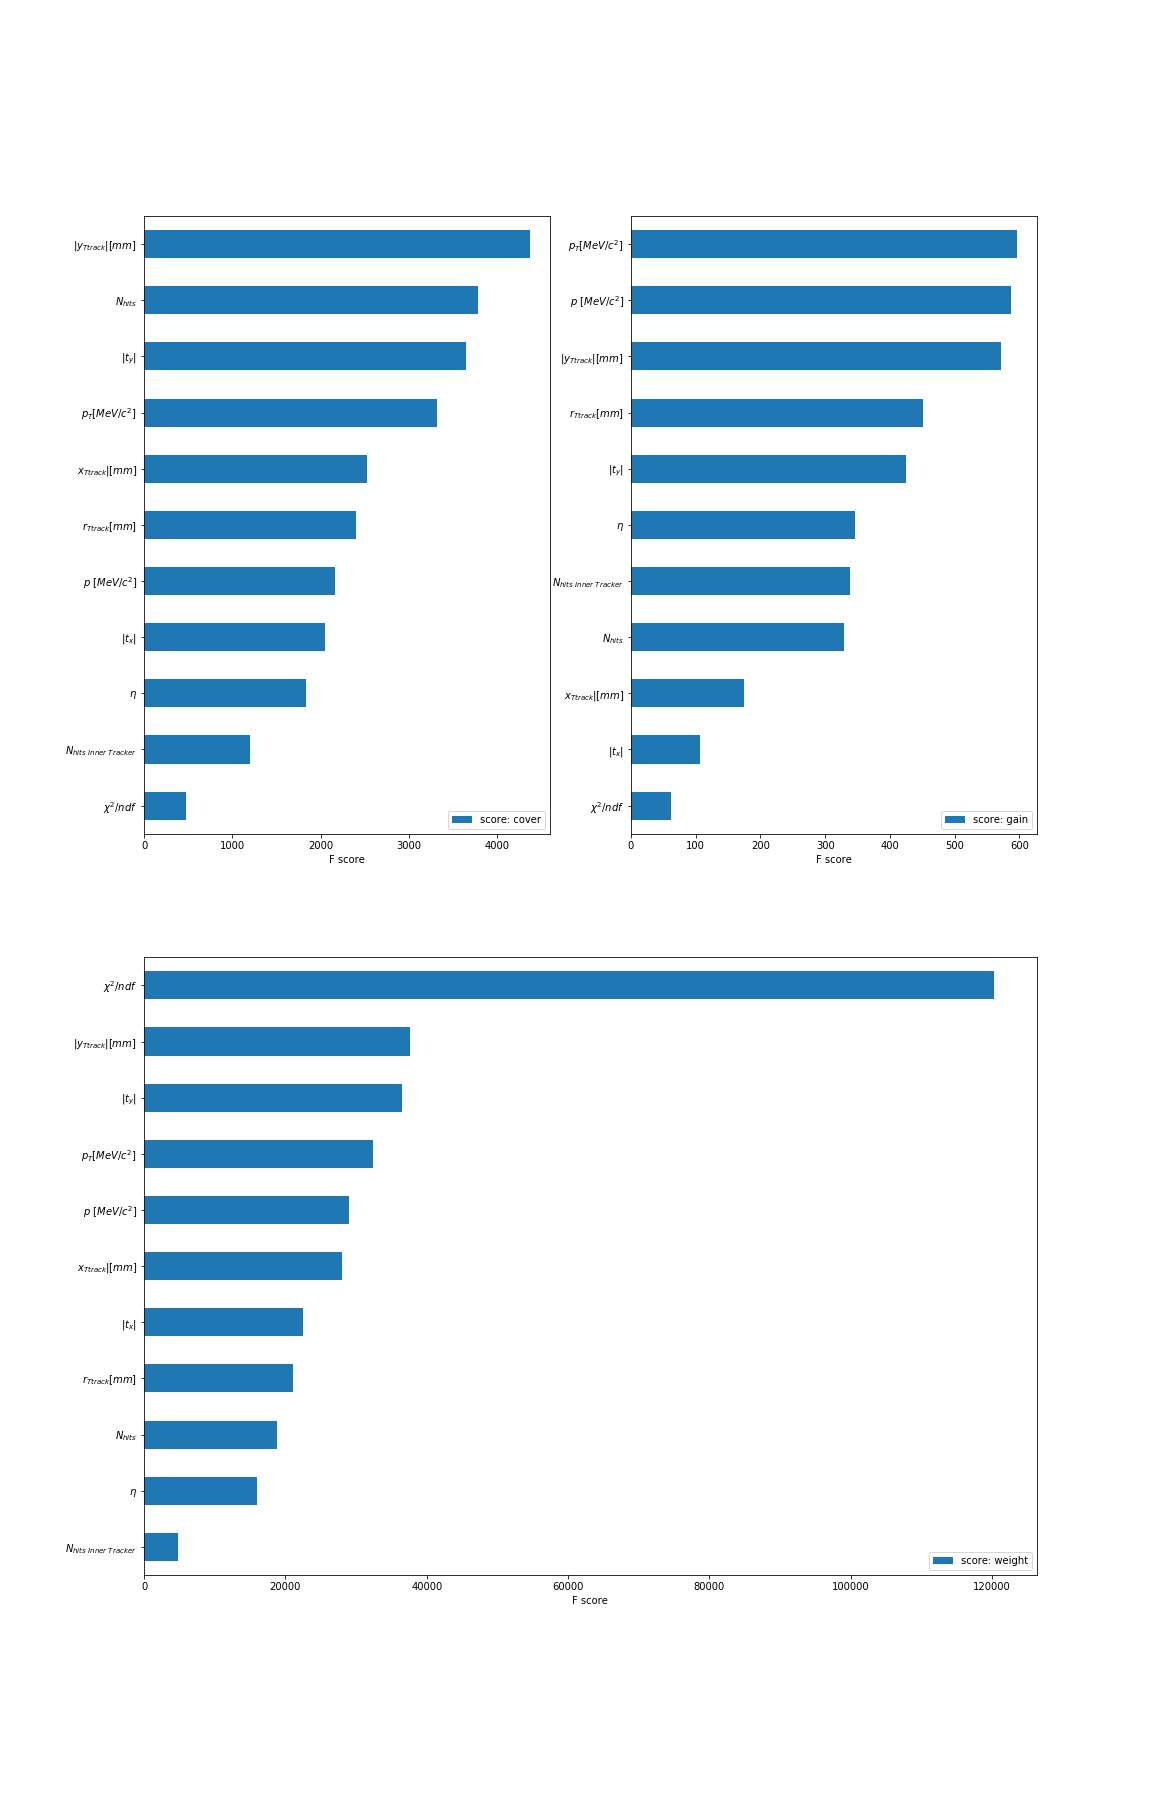
\includegraphics[scale=0.8]{figures/feature_importance.png}
\caption{Feature Importance plots for XGBoost model. Each of the plots were obtained for a different global feature importance metrics: coverage (upper left), gain (upper right) and weight (bottom). 
\label{fig:xgboost overal features importance}}
\end{figure}

The second method to take a closer look inside the xgboost black box is based on the idea of Shapley value, described in section [??]. The analysis of the importance of the features is usually done by presenting two groups of plots. The first group is presented in figure \ref{fig:shap overall}. The standardized importance plot provides a notion of relative feature importance and can be compared with the classical plots described previously. Although, it doesn't provide any additional information on the distribution of impacts that feature has on the model's output. This plot doesn't give any understanding of the feature's value on the model performance  \cite{Shap2}. To overcome this limitation the Shap summary plot was introduced, which leverages individualized feature attribution to the model's decision. In order to make that kind of plot the features are sorted by their global impact $\sum_{j=1}^{N}|\phi_i^{(j)}|$, then each of the dots corresponding to the Shap values $\phi_i^{(j)}|$ are plotted horizontally, stacked vertically when running out of space. This concept allows achieving similar effect to the violin plots, which can be further enhanced by coloring the dots according to the feature's value. 


\begin{figure}
\begin{subfigure}
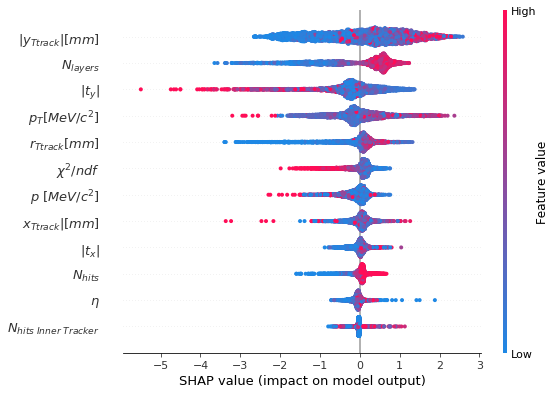
\includegraphics[width=\linewidth]{figures/Shap_overall.png}
\end{subfigure}
\hfill
\begin{subfigure}
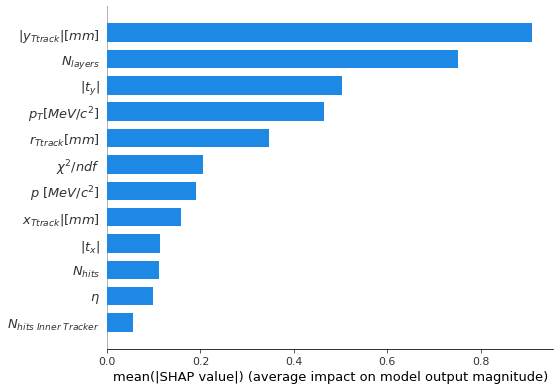
\includegraphics[width=\linewidth]{figures/Shap_mean.png}
\end{subfigure}%
   \caption{Shap summary plots of all T-Seed classifier features. The plots were obtained using a sample of 50 thousand test examples. The interpretation of this plot is straightforward, the higher Shap value of the feature, the higher influence on the decision of whether T-Seed is reconstructable. In the upper plot, each dot represents every feature for every individual test example that was run through the model. Dot's are colored by the feature's value (red high, blue low). The bottom plot presents the standard feature importance bar plot. The x-axis is essentially the average magnitude change in model output when a feature is hidden from the model.}  
\label{fig:shap overall}
\end{figure}


To get a better understanding of Shap values presented in the figure \ref{fig:shap overall} let focus on one feature - $N_{layers}$. It is the second most important feature to decide whether T-Seed is a ghost. The impact of this feature on a model's output varies smoothly as the value of the feature increases, which is indicated by the smooth color gradient. The long tail reaching the left means that the extreme values of these features can significantly increase the probability that this T-Seed is not a valid seed. This is consistent with priory intuition saying the seed, that was reconstructed using a small number of hits are more likely to be a ghost. 

The second type of Shap based plots is dependence plots presented in figure \ref{fig:shap dep}.  The concept is similar to the pair-plot, which are usually created in order to visualize dependencies between two features. The shap dependence plots also take into consideration the Shap values. The idea is to make a scatter plot, shap value versus feature value, and apply color scheme that is based on the value of the second feature.

The plot (a) is the one that is the easiest to interpret. It shows the shap value versus the number of layers. It is clearly visible that T tracks with the numbers of plates smaller than 15 push strongly the classifier toward negative decisions. This effect is escalated when the track has a big value of $\chi^2 /\ dof $. This means the classifier decision agreed with an initial understanding of the problem, the track that was reconstructed using a small number of hits and it's fit to the track model has a poor quality is more likely to be a ghost. 


\begin{figure}[tbph]
\begin{center}
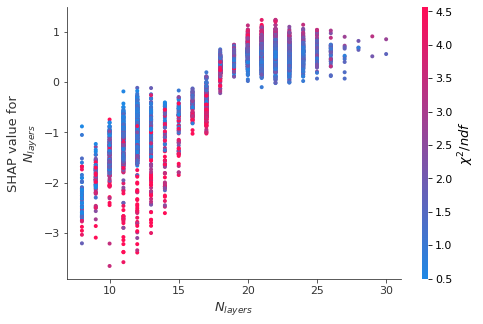
\includegraphics[width = 0.49\textwidth]{figures/dependence_plot3.png} 
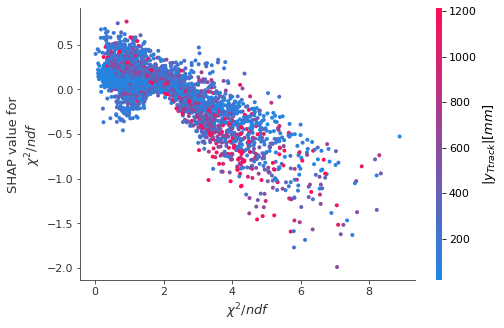
\includegraphics[width = 0.49\textwidth]{figures/dependence_plot1.png} \\
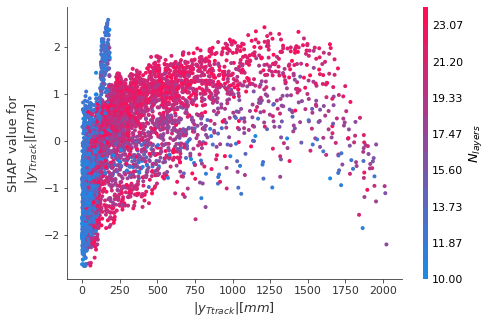
\includegraphics[width = 0.49\textwidth]{figures/dependence_plot2.png} 
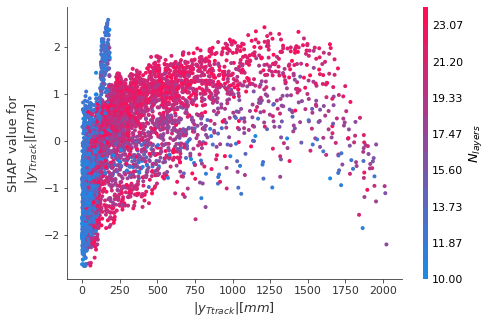
\includegraphics[ width = 0.49\textwidth]{figures/dependence_plot2.png} \\
   \caption{Shap dependence plots. Each dot is a track. The x-axis shows the value of the \textbf{feature 1} and the y-axis is the Shap value attributed to this feature. To show the dependence between \textbf{feature 1} and \textbf{feature 2} the color of particular dot depends of the value of the \textbf{feature 2}. }
   \label{fig:shap dep}
 \end{center}
 \end{figure}

The result of the evaluation of the third and final approach, the one that is base on LIME model, is shown in figure \ref{fig:limeResult}. The presented LIME outcome ware obtained for two randomly chosen test examples. Each of these examples represents one of the target classes. It provides a good indication of the importance of the features and highlights why particular decision was made. The length of each bar is proportional to the feature's value times linear regression weight associated with this feature.  It is easy to notice, that one of the most important feature is the number of hits, that were used to reconstruct T-Seeds and this is consistent with the initial intuition.  

\begin{figure}
\begin{subfigure}
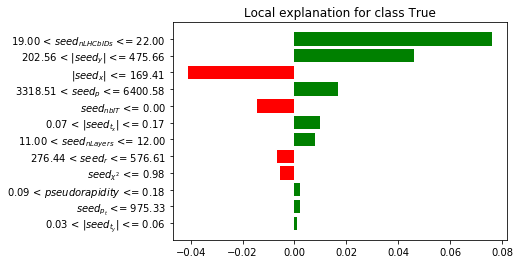
\includegraphics[width=\linewidth]{figures/LIME_true.png}
\caption{LIME explanation for randomly chosen True example  }
\end{subfigure}
\hfill
\begin{subfigure}
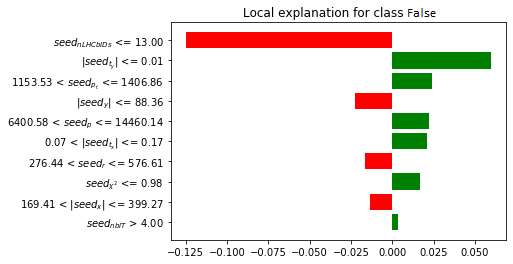
\includegraphics[width=\linewidth]{figures/lime_ghost.png}
\caption{LIME explanation for randomly chosen Ghost example}
\end{subfigure}%
\caption{Exemplary outcome of the LIME for two randomly chosen examples. Those samples were drown from the test dataset. 
The red color indicates that the features pushed prediction toward ghost. 
}\label{fig:limeResult}
\end{figure}




\section{Physics Performance of the modernised downstream tracking}
\label{sec:physic_performance}
The previous sections describe the LongLived pattern recognition algorithm. This one is dedicated to showing the physics performance of this algorithm. The performance can be measured using various strategies. The most obvious one is to measure the efficiency of reconstructing a charged particle in the acceptance as a downstream track using Monte Carlo simulated samples.
The second method uses to evaluate the performance using real data. This method determines and compares the pattern recognition algorithm performance by measuring the mass resolution.  

\subsection{Monte Carlo based Downstream Tracking efficiency  }

The pattern recognition algorithm performance measurement can be determined from Monte Carlo simulations by comparing the number of track that the algorithm managed to find (reconstructed tracks) with the maximum number of track that it could possibly find (reconstructable tracks). This section is based on the one \cite{PATLLT}. 

To discuss the efficiency of the pattern recognition algorithm it is obligatory to define a number of quantities that are used in this study.  First of all, the MC particle is said to be \textbf{reconstructible}, if it left the sufficient number of hits in the detector. The particle reconstructible criteria vary for one subdetector to another, and they are summarized \cite{track_def}:

\begin{itemize}
    \item Velo reconstructible is a particle that has at least three hits in $R$ and $\varphi$ sensors.
    \item TT reconstructible particle is consider when it has at least one hit in the first two planes (TTa) and one hit in the last tow planes (TTb). 
    \item T-Station reconstructible is a particle that has at least one x and one stereo hit in each of the three T-Stations. 
\end{itemize}

Therefore the definition of particle reconstructible as a Downstream track if it satisfies the TT and T-Stations reconstructibility criteria. In order to associate the reconstructed tracks to the reconstructable ones a cross-check of hits in both of them has to be evaluated. A reconstructed track is considered as matched to a simulated Monte Carlo particle if they share at least 70\% of the hits.  
Based on this definition the following pattern recognition performance metrics can be defined: 

\begin{itemize}
    \item The \textbf{Tracking efficiency} ($\varepsilon$) is defined as a ratio between the amount od reconstructed and matched track to the total amount of reconstructable tracks. 
    \begin{equation}
        \varepsilon  = \frac{\textrm{reconstructed} \cap  \textrm{matched}}{\textrm{reconstructable}}
    \end{equation}
    \item The \textbf{ghost rate} is the amount of reconstructed tracks not associated to any of the Monte Carlo particle, thus having less than 70\% of matched hits, with respect to the total amount of tracks found by the pattern recognition algorithm
    \begin{equation}
       \textrm{ghost rate} =  \frac{\textrm{not matched}}{\textrm{reconstructable}}
    \end{equation}
\end{itemize}

 Within the scope of this analysis the efficiency of a Downstream Tracking algorithm is calculated as the one that includes the efficiency of a Long-Lived Tracking pattern recognition algorithm combined together with the efficiency of the T-Seed reconstruction.

In the presented studies, the analysis was performed on a sample constituted of 50,000 simulated events of both magnet polarities. Two types of decays were simulated: $B^{0} \rightarrow J/\Psi K^{0}_{S}$ and $D^{*+} \rightarrow D^{0}\pi^+$. The first type of decay was selected to represent $B$ meson decays and the second one for a charm. 
There are four different categories of track that were considered within the scope of this performance analysis on MC data:

\begin{itemize}
    \item $\varepsilon_{TT+T}$ : efficiency for all downstream reconstructible particles;
    \item $\varepsilon_{TT+T, p>5Gev/c}$ : efficiency for all downstream reconstructible particles with $p> 5 GeV/c$;
    \item $\varepsilon_{TT+T, from B/D}$ : efficiency for all downstream reconstructible particles from a decay of $B$ or $D$ meson;
    \item $\varepsilon_{TT+T, from B/D, p>5 GeV }$ : efficiency for all downstream reconstructible particles from a decay of $B$ or $D$ meson with  $p> 5 GeV/c$.;
\end{itemize}

The overall efficiency numbers are collected in upper half of Table \ref{table:overall eff} and the ghost rate related numbers are presented in \ref{tab:overall ghost} (upper half). Plots of the efficiency and the ghost rate as a function of momentum, transverse momentum, and pseudorapidity are shown in 
figures \ref{fig:EffPatLLTBJpsiK}, \ref{fig:ghostPatLLTBJpsiK}  (obtained using  $B^{0} \rightarrow J/\Psi K^{0}_{S}$ ) and \ref{fig:EffPatLLTDstD0pi}, \ref{fig:ghostsPatLLTDstD0pi} (for $D^{*+} \rightarrow D^{0}\pi^+$ decay). No uncertainty is given, because presented numbers were obtained on a Monte Carlo samples not on a collision data. The statistical uncertainty are negligible, at the permille level.  

It was also important to measure the downstream tracking efficiency using the samples that were fitted with Kalman Filter and a quality cut on a $\chi^2\/ndf$ was applied. Those tracks were also proceeded by a clone killing algorithm to remove duplicates, which were reconstructed as long and downstream track simultaneously. The performance numbers referring to those tracks are collected in Table \ref{tab:overall eff}, lower half, and Table \ref{tab:overall ghost} (lower half) gives ghost rates. The performance numbers after these three steps seem worse than before, as the processing steps applied also reject correct tracks, and the cloned killer is inefficient. One of the reasons why it happens, the clon killer sometimes falsely classifies downstream tracks as long
tracks (for example when the Velo part is a ghost), which then gets removed from the downstream statistics. Furthermore, clone killing prefers long tracks over downstream tracks. 

Downstream tracking efficiency strongly depends on the momentum and transverse momentum of the tracks. The explanation of the phenomenon can be based on factors such as the search windows do not cover the full region necessary to find all tracks. Secondly, for low momentum tracks, search windows are generally larger than for high momentum tracks, which increases the number of hits in the search window, and increases the chances that the pattern recognition identifies the wrong hits.

In addition, the downstream tracks that were also reconstructed as long tracks
are less prone to be ghosts, which is why the ghost fraction actually increases
after the Kalman Filter, the clone killer and the ghost probability cut. However, it should be noted that
in a physics analysis of a decay channel, a strict cut is normally placed on the ghost probability of the downstream tracks, which reduces the ghost fraction
significantly.


\begin{table}[htp]
\caption{Reconstruction efficiency of downstream tracks on simulated samples of
$B^{0} \rightarrow J/\Psi K^{0}_{S}$ and $D^{*+} \rightarrow D^{0}\pi^+$ decays. The upper half are non-filtered tracks, the lower half is after the clone killer, Kalman Filter and ghost probability. This efficiency
includes the efficiency of T-Seed reconstruction and LongLived Tracking. Due to a softer
momentum spectrum, the efficiency is lower in the$D^{*+} \rightarrow D^{0}\pi^+$
sample.}
\begin{center}
\begin{tabular}{c|c|c|c|c|c}
filter & decay type & $\varepsilon_{TT+T}$ & $\varepsilon_{TT+T, ~p>5 GeV}$ & $\varepsilon_{TT+T\text{, from} B/D}$ & $\varepsilon_{TT+T\text{, from} B/D, ~p>5 GeV}$ \\
\hline
No &$B^{0} \rightarrow J/\Psi K^{0}_{S}$  & 73.3\% & 80.1\% & 81.4\% & 85.4\%\\
No &  $D^{*+} \rightarrow D^{0}\pi^+$ & 71.3\% & 78.0\% & 76.8\% & 81.4\% \\
\hline
Yes & $B^{0} \rightarrow J/\Psi K^{0}_{S}$  & 70.0\% & 76.7\% & 79.0\% & 83.2\% \\
Yes & $D^{*+} \rightarrow D^{0}\pi^+$ & 67.3\% & 73.7\% & 73.1\% & 77.3\%
\end{tabular}
\end{center}
\label{tab:overall eff}
\end{table}%

%%%%%%%%%%%%%%%%%%%%%%%%%%%%%%%%%%%%%%%%%%%%%%%%%%%%%%%%%%
\begin{table}[htp]
\caption{Ghost fraction of downstream tracks on simulated samples of
$B^{0} \rightarrow J/\Psi K^{0}_{S}$ and $D^{*+} \rightarrow D^{0}\pi^+$ decays. The upper half are non-filtered tracks, the lower half is after the clone killer, Kalman Filter and ghost probability. This ghost fraction
includes the ghosts produced in T-Seed pattern Recognition and Long-Lived Tracking. Due to a
softer momentum spectrum, the ghost fraction is higher in the
 $D^{*+} \rightarrow D^{0}\pi^+$ sample.}
\begin{center}
\begin{tabular}{c|c|c}
filter & decay type & fraction of ghosts \\
\hline
No & $B^{0} \rightarrow J/\Psi K^{0}_{S}$ & 29.5\% \\
No & $D^{*+} \rightarrow D^{0}\pi^+$ & 30.3\% \\
\hline
yes &$B^{0} \rightarrow J/\Psi K^{0}_{S}$ & 39.2\% \\
yes & $D^{*+} \rightarrow D^{0}\pi^+$ & 40.2\% \\
\end{tabular}
\end{center}
\label{tab:overall ghost}
\end{table}%



\begin{figure}[tbph]
\begin{center}
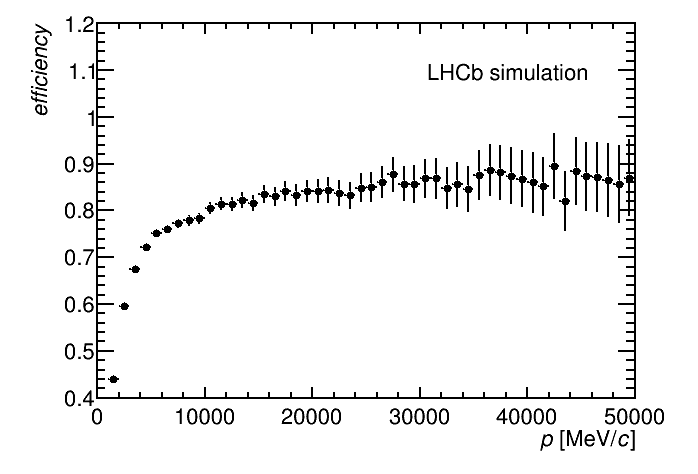
\includegraphics[width = 0.49\textwidth]{figures/EffPatLLT/overall/BJpsiKSP.png}
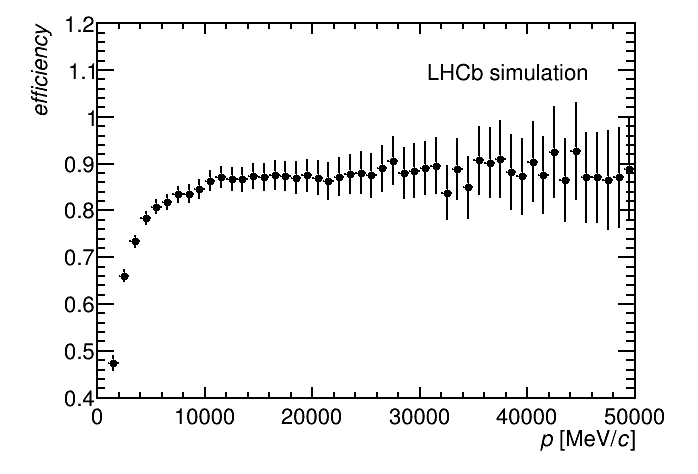
\includegraphics[width = 0.49\textwidth]{figures/EffPatLLT/overall/BJpsiKSFromBDP.png}
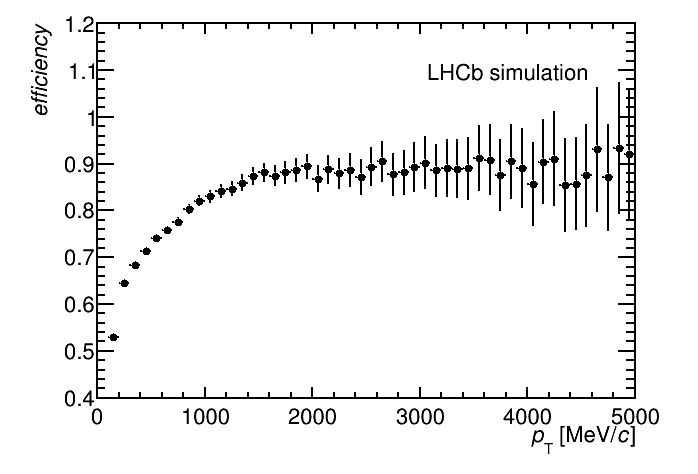
\includegraphics[width = 0.49\textwidth]{figures/EffPatLLT/overall/BJpsiKSPt.png}
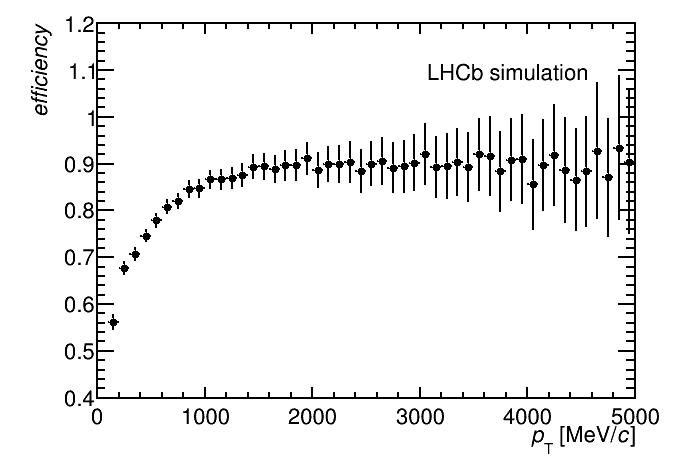
\includegraphics[width = 0.49\textwidth]{figures/EffPatLLT/overall/BJpsiKSFromBDPt.png}
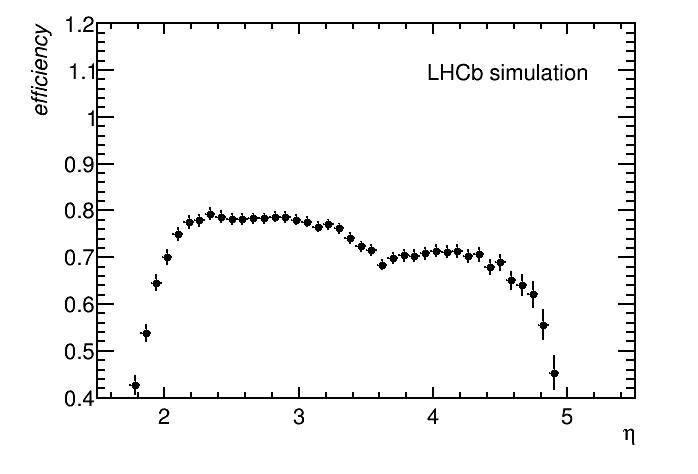
\includegraphics[width = 0.49\textwidth]{figures/EffPatLLT/overall/BJpsiKSEta.png}
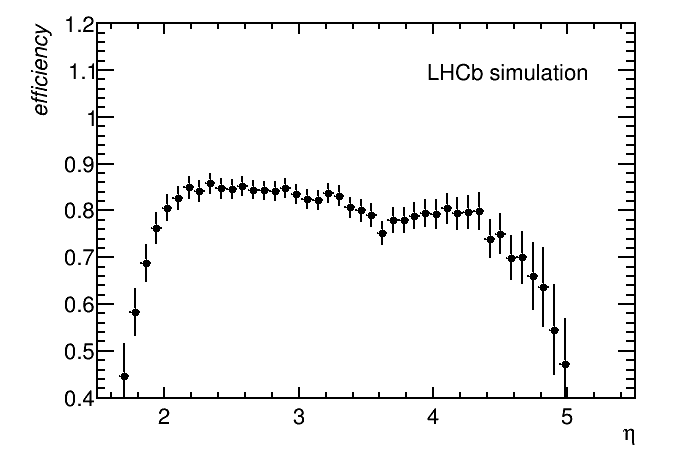
\includegraphics[width = 0.49\textwidth]{figures/EffPatLLT/overall/BJpsiKSFromBDEta.png}
\caption{Efficiencies to reconstruct downstream tracks as a function of momentum
(top row), transverse momentum (middle row) and pseudorapidity (bottom row). The
left column is for all downstream reconstructible tracks, the right column for
all downstream tracks from a decay chain of a $B$ or $D$ meson. The efficiencies are
obtained on a simulated sample of  $B^{0} \rightarrow J/\Psi K^{0}_{S}$ decays.}
\label{fig:EffPatLLTBJpsiK}
 \end{center}
\end{figure}
%%%%%%%%%%%%%%%%%%%%%%%%%%%%%%%%%%%%%%%%%%%%%%%%%%%%%%%%%%
\begin{figure}[tbph]
\begin{center}
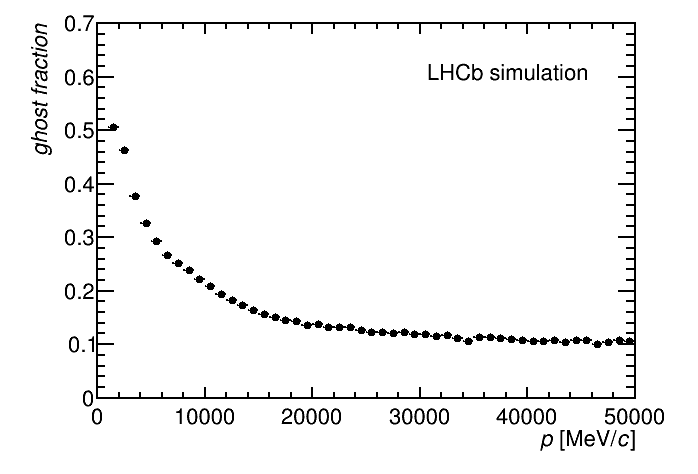
\includegraphics[width = 0.49\textwidth]{figures/EffPatLLT/overall/BJpsiKSGhostFracP.png}
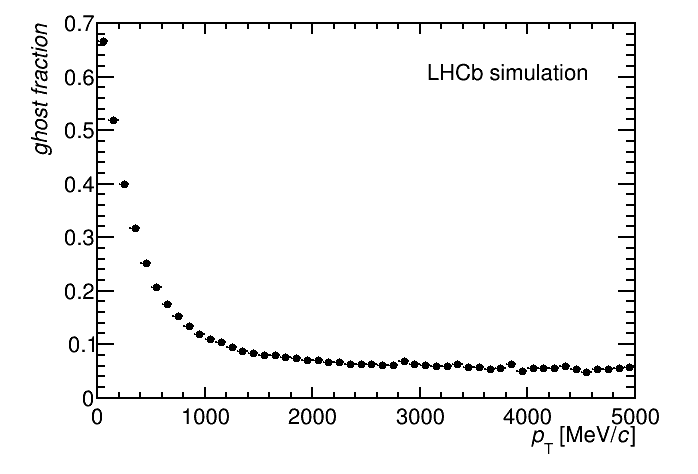
\includegraphics[width = 0.49\textwidth]{figures/EffPatLLT/overall/BJpsiKSGhostFracPt.png}
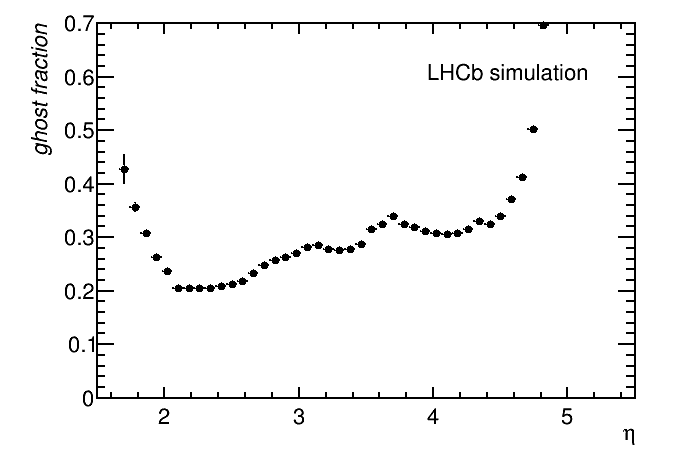
\includegraphics[width = 0.49\textwidth]{figures/EffPatLLT/overall/BJpsiKSGhostFracEta.png}
\caption{Ghost fraction in downstream tracks as a function of momentum (top
left), transverse momentum (top right) and pseudorapidity (bottom). The ghost
fractions are obtained on a simulated sample of  $B^{0} \rightarrow J/\Psi K^{0}_{S}$ decays.}
\label{fig:ghostPatLLTBJpsiK}
 \end{center}
 \end{figure}
%%%%%%%%%%%%%%%%%%%%%%%%%%%%%%%%%%%%%%%%%%%%%%%%%%%%%%%%%%
\begin{figure}[tbph]
\begin{center}
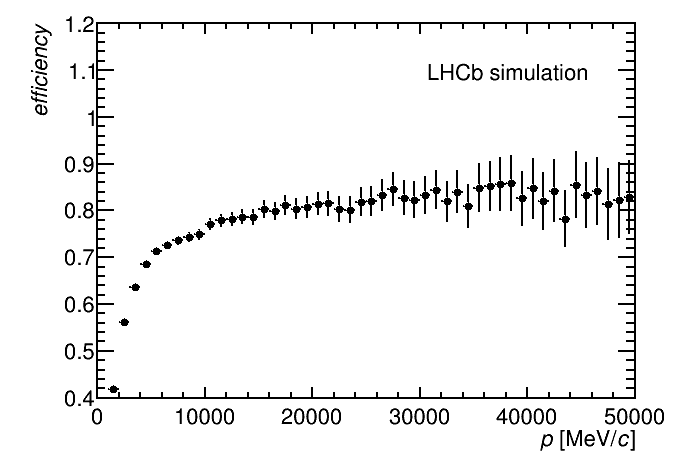
\includegraphics[width = 0.49\textwidth]{figures/EffPatLLT/overall/BJpsiKSP_TBTC.png}
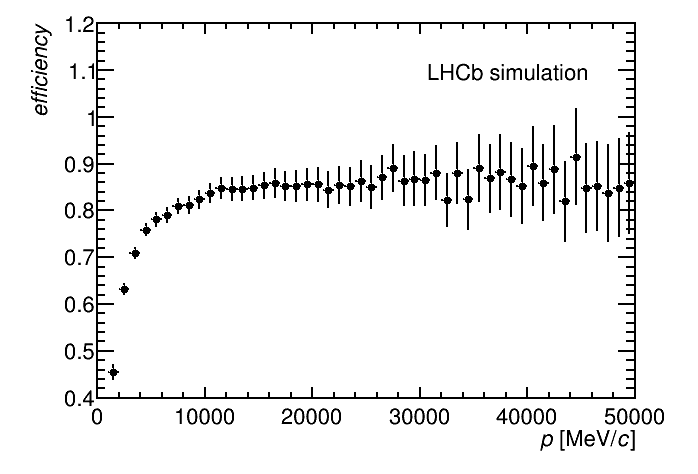
\includegraphics[width = 0.49\textwidth]{figures/EffPatLLT/overall/BJpsiKSFromBDP_TBTC.png}
\includegraphics[width = 0.49\textwidth]{figures/EffPatLLT/overall/BJpsiKSPt_TBTC.png}
\includegraphics[width = 0.49\textwidth]{figures/EffPatLLT/overall/BJpsiKSFromBDPt_TBTC.png}
\includegraphics[width = 0.49\textwidth]{figures/EffPatLLT/overall/BJpsiKSEta_TBTC.png}
\includegraphics[width = 0.49\textwidth]{figures/EffPatLLT/overall/BJpsiKSFromBDEta_TBTC.png}
\caption{Efficiencies to reconstruct downstream tracks, after clone killing,
Kalman filtering and the cut on the ghost probability, as a function of momentum
(top row), transverse momentum (middle row) and pseudorapidity (bottom row). The
left column is for all downstream reconstructible tracks, the right column for
all downstream tracks from a decay chain of a $B$ or $D$ meson. The efficiencies are
obtained on a simulated sample of  $B^{0} \rightarrow J/\Psi K^{0}_{S}$ decays.}
\label{fig:EffPatLLTBJpsiK_TBTC}
 \end{center}
 \end{figure}
%%%%%%%%%%%%%%%%%%%%%%%%%%%%%%%%%%%%%%%%%%%%%%%%%%%%%%%%%%
\begin{figure}[tbph]
\begin{center}
\includegraphics[width = 0.49\textwidth]{figures/EffPatLLT/overall/BJpsiKSGhostFracP_TBTC.png}
\includegraphics[width = 0.49\textwidth]{figures/EffPatLLT/overall/BJpsiKSGhostFracPt_TBTC.png}
\includegraphics[width = 0.49\textwidth]{figures/EffPatLLT/overall/BJpsiKSGhostFracEta_TBTC.png}
\caption{Ghost fraction in downstream tracks, after clone killing, Kalman
filtering and the cut on the ghost probability, as a function of momentum (top
left), transverse momentum (top right) and pseudorapidity (bottom). The ghost
fractions are obtained on a simulated sample of $B^{0} \rightarrow J/\Psi K^{0}_{S}$ decays.}
\label{fig:ghostPatLLTBJpsiK_TBTC}
 \end{center}
 \end{figure}


\begin{figure}[tbph]
\begin{center}
\includegraphics[width = 0.49\textwidth]{figures/EffPatLLT/overall/DstD0piP.png} 
\includegraphics[width = 0.49\textwidth]{figures/EffPatLLT/overall/DstD0piFromBDP.png}
\includegraphics[width = 0.49\textwidth]{figures/EffPatLLT/overall/DstD0piPt.png} 
\includegraphics[width = 0.49\textwidth]{figures/EffPatLLT/overall/DstD0piFromBDPt.png}
\includegraphics[width = 0.49\textwidth]{figures/EffPatLLT/overall/DstD0piEta.png} 
\includegraphics[width = 0.49\textwidth]{figures/EffPatLLT/overall/DstD0piFromBDEta.png}
\caption{Efficiencies to reconstruct downstream tracks as a function of momentum (top row), transverse momentum (middle row) and pseudorapidity (bottom row). The left column is for all downstream reconstructible tracks, the right column for all downstream tracks from a decay chain of a $B$ or $D$ meson. The efficiencies are obtained on a simulated sample of$D^{*+} \rightarrow D^{0}\pi^+$ decays.}
\label{fig:EffPatLLTDstD0pi}
 \end{center}
 \end{figure}

\begin{figure}[tbph]
\begin{center}
\includegraphics[width = 0.49\textwidth]{figures/EffPatLLT/overall/DstD0piP_TBTC.png} 
\includegraphics[width =0.49\textwidth]{figures/EffPatLLT/overall/DstD0piFromBDP_TBTC.png}
\includegraphics[width = 0.49\textwidth]{figures/EffPatLLT/overall/DstD0piPt_TBTC.png} 
\includegraphics[width =0.49\textwidth]{figures/EffPatLLT/overall/DstD0piFromBDPt_TBTC.png}
\includegraphics[width = 0.49\textwidth]{figures/EffPatLLT/overall/DstD0piEta_TBTC.png} 
\includegraphics[width =0.49\textwidth]{figures/EffPatLLT/overall/DstD0piFromBDEta_TBTC.png}
\caption{Efficiencies to reconstruct downstream tracks, after clone killing, Kalman filtering and the cut on the ghost probability, as a function of momentum (top row), transverse momentum (middle row) and pseudorapidity (bottom row). The left column is for all downstream reconstructible tracks, the right column for all downstream tracks from a decay chain of a $B$ or $D$ meson. The efficiencies are obtained on a simulated sample of $D^{*+} \rightarrow D^{0}\pi^+$ decays.}
\label{fig:EffPatLLTDstD0p_TBTCi}
 \end{center}
 \end{figure}

\begin{figure}[tbph]
\begin{center}
\includegraphics[width=0.49\textwidth]{figures/EffPatLLT/overall/DstD0piGhostFracP.png} 
\includegraphics[width=0.49\textwidth]{figures/EffPatLLT/overall/DstD0piGhostFracPt.png}
\includegraphics[width=0.49\textwidth]{figures/EffPatLLT/overall/DstD0piGhostFracEta.png} 
\caption{Ghost fraction in downstream tracks as a function of momentum (top left), transverse momentum (top right) and pseudorapidity (bottom). The ghost fractions are obtained on a simulated sample of $D^{*+} \rightarrow D^{0}\pi^+$ decays.}
\label{fig:ghostsPatLLTDstD0pi}
 \end{center}
 \end{figure}

\begin{figure}[tbph]
\begin{center}
\includegraphics[width =0.49\textwidth]{figures/EffPatLLT/overall/DstD0piGhostFracP_TBTC.png} 
\includegraphics[width =0.49\textwidth]{figures/EffPatLLT/overall/DstD0piGhostFracPt_TBTC.png}
\includegraphics[width =0.49\textwidth]{figures/EffPatLLT/overall/DstD0piGhostFracEta_TBTC.png} 
\caption{Ghost fraction in downstream tracks, after clone killing, Kalman filtering and the cut on the ghost probability, as a function of momentum (top left), transverse momentum (top right) and pseudorapidity (bottom). The ghost fractions are obtained on a simulated sample of $D^{*+} \rightarrow D^{0}\pi^+$ decays.}
\label{fig:ghostsPatLLTDstD0pi_TBTC}
 \end{center}
 \end{figure}


\subsection{Comparison between Long-Lived Tracking algorithm and its predecessor}
The analysis presented within this section is dedicated to comparing the performance of the Long-Lived Tracking algorithm and its predecessor called PatDownstream \cite{PatDownstream}. The corresponding performance numbers are given in tables \ref{tab:PatLLTPatDownstreamEffComp} \ref{tab:PatLLTPatDownstreamEffCompTBTC} \ref{tab:globGhostComp}. 

Figures \ref{} \ref{ } show the efficiency and ghost rates of downstream tracks reconstructed via these two algorithms as a function of momentum, transverse momentum, and pseudorapidity. Those plots visualize tracking algorithm performance that was obtained using a simulated sample of B  and no other processing was applied. 

Figures \ref{} \ref{} present the same quantities, after Kalman filtering and clone killer. 
It is clearly visible, that the performance gain and the strong reduction of ghost rates were measured for the new algorithm. It is presumed that the significant ghost rate reduction (about 16\%) was achieved due to the good performance of the T-Seed classifier, which was one of the major goals of the author’s study. 


\begin{table}[htp]
\caption{Comparions of reconstruction efficiency of downstream tracks made with Long-Lived Tracking algorithm or PatDownstream, on simulated samples of $B^{0} \rightarrow J/\Psi K^{0}_{S}$ . This efficiency includes the efficiency of PatSeeding and Long-Lived Tracking algorithm.}
\begin{center}
\begin{tabular}{c|c|c|c|c}
algorithm & $\varepsilon_{TT+T}$ & $\varepsilon_{TT+T, ~p>5 GeV}$ & $\varepsilon_{TT+T\text{, from} B/D}$ & $\varepsilon_{TT+T\text{, from} B/D, ~p>5 GeV}$ \\
\hline 
Long-Lived Tracking & 73.3\% & 80.1\% & 81.4\% & 85.4\%\\
PatDownstream          & 68.3\% & 74.4\% & 77.1\% & 81.6\% 
\end{tabular}
\end{center}
\label{tab:PatLLTPatDownstreamEffComp}
\end{table}%

\begin{table}[htp]
\caption{Comparions of reconstruction efficiency of downstream tracks made with PatLongLivedTracking or PatDownstream, on simulated samples of $B^{0} \rightarrow J/\Psi K^{0}_{S}$, after the Kalman Filter and clone killer. This efficiency includes the efficiency of PatSeeding and PatLongLivedTracking. The efficiency decreases compared to Table~\ref{tab:PatLLTPatDownstreamEffComp} due to inefficiency of the clone killer.}
\begin{center}
\begin{tabular}{c|c|c|c|c}
algorithm & $\varepsilon_{TT+T}$ & $\varepsilon_{TT+T, ~p>5 GeV}$ & $\varepsilon_{TT+T\text{, from} B/D}$ & $\varepsilon_{TT+T\text{, from} B/D, ~p>5 GeV}$ \\
\hline 
Long-Lived Tracking & 70.0\% & 76.7\% & 79.0\% & 83.2\% \\
PatDownstream          & 63.7\% & 71.3\% & 74.5\% & 79.2\% 
\end{tabular}
\end{center}
\label{tab:PatLLTPatDownstreamEffCompTBTC}
\end{table}%

\begin{table}[htp]
\caption{Ghost fraction of downstream tracks on simulated samples of $B^{0} \rightarrow J/\Psi K^{0}_{S}$ for PatLongLivedTracking and PatDownstream, once before and after the clone killer, Kalman Filter and ghost probability (CKG) were applied. This ghost fraction includes the ghosts produced in PatSeeding and PatLongLivedTracking (PatDownstream). The ghost fraction is higher after the clone killer as tracks, also reconstructed as long tracks, are not present in that number.}
\begin{center}
\begin{tabular}{c|c|c}
algorithm & fraction of ghosts & fraction of ghosts after CKG \\
\hline 
Long-Lived Tracking & 29.5\% & 39.2\%\\
PatDownstream & 46.3\% & 52.1\% \\
\end{tabular}
\end{center}
\label{tab:globGhostComp}
\end{table}%



%%%%%%%%%%%%%%%%%%%%%%%%%%%%%%%%%%%%%%

\begin{figure}[tbph]
\begin{center}
\includegraphics[width = 0.49\textwidth]{figures/EffPatLLT/compare/BJpsiKSP.png} 
\includegraphics[width = 0.49\textwidth]{figures/EffPatLLT/compare/BJpsiKSFromBDP.png}
\includegraphics[width = 0.49\textwidth]{figures/EffPatLLT/compare/BJpsiKSPt.png} 
\includegraphics[width = 0.49\textwidth]{figures/EffPatLLT/compare/BJpsiKSFromBDPt.png}
\includegraphics[width = 0.49\textwidth]{figures/EffPatLLT/compare/BJpsiKSEta.png} 
\includegraphics[width = 0.49\textwidth]{figures/EffPatLLT/compare/BJpsiKSFromBDEta.png}
\caption{Efficiencies to reconstruct downstream tracks as a function of momentum (top row), transverse momentum (middle row) and pseudorapidity (bottom row), in red for Long-Lived Tracking algorithm and in black for PatDownstream. The left column is for all downstream reconstructible tracks, the right column for all downstream tracks from a decay chain of a $B$ or $D$ meson. The efficiencies are obtained on a simulated sample of  $B^{0} \rightarrow J/\Psi K^{0}_{S}$ decays.}
\label{fig:EffCompPatLLTBJpsiK}
 \end{center}
 \end{figure}

\begin{figure}[tbph]
\begin{center}
\includegraphics[width = 0.49\textwidth]{figures/EffPatLLT/compare/BJpsiKSGhostFracP.png} 
\includegraphics[width = 0.49\textwidth]{figures/EffPatLLT/compare/BJpsiKSGhostFracPt.png}
\includegraphics[width = 0.49\textwidth]{figures/EffPatLLT/compare/BJpsiKSGhostFracEta.png} 
\caption{Ghost fraction in downstream tracks as a function of momentum (top left), transverse momentum (top right) and pseudorapidity (bottom), in red for Long-Lived Tracking algorithm and in black for PatDownstream. The ghost fractions are obtained on a simulated sample of $B^{0} \rightarrow J/\Psi K^{0}_{S}$ decays.}
\label{fig:ghostCompPatLLTBJpsiK}
 \end{center}
 \end{figure}

%%%%%%%%%%%%%%
%%%%%%%%%%%%%%

\begin{figure}[tbph]
\begin{center}
\includegraphics[width = 0.49\textwidth]{figures/EffPatLLT/compare/BJpsiKSP_TBTC.png} 
\includegraphics[width = 0.49\textwidth]{figures/EffPatLLT/compare/BJpsiKSFromBDP_TBTC.png}
\includegraphics[width = 0.49\textwidth]{figures/EffPatLLT/compare/BJpsiKSPt_TBTC.png} 
\includegraphics[width = 0.49\textwidth]{figures/EffPatLLT/compare/BJpsiKSFromBDPt_TBTC.png}
\includegraphics[width = 0.49\textwidth]{figures/EffPatLLT/compare/BJpsiKSEta_TBTC.png} 
\includegraphics[width = 0.49\textwidth]{figures/EffPatLLT/compare/BJpsiKSFromBDEta_TBTC.png}
\caption{Efficiencies to reconstruct downstream tracks, after clone killing, Kalman filtering and the cut on the ghost probability, as a function of momentum (top row), transverse momentum (middle row) and pseudorapidity (bottom row). The left column is for all downstream reconstructible tracks, the right column for all downstream tracks from a decay chain of a $B$ or $D$ meson. The efficiencies are obtained on a simulated sample of  $B^{0} \rightarrow J/\Psi K^{0}_{S}$ decays.}
\label{fig:EffCompPatLLTBJpsiK_TBTC}
 \end{center}
 \end{figure}

\begin{figure}[tbph]
\begin{center}
\includegraphics[width = 0.49\textwidth]{figures/EffPatLLT/compare/BJpsiKSGhostFracP_TBTC.png} 
\includegraphics[width = 0.49\textwidth]{figures/EffPatLLT/compare/BJpsiKSGhostFracPt_TBTC.png}
\includegraphics[width = 0.49\textwidth]{figures/EffPatLLT/compare/BJpsiKSGhostFracEta_TBTC.png} 
\caption{Ghost fraction in downstream tracks, after clone killing, Kalman filtering and the cut on the ghost probability, as a function of momentum (top left), transverse momentum (top right) and pseudorapidity (bottom). The ghost fractions are obtained on a simulated sample of  $B^{0} \rightarrow J/\Psi K^{0}_{S}$ decays.}
\label{fig:ghostCompPatLLTBJpsiK_TBTC}
 \end{center}
 \end{figure}

\subsection{Performance measured using collision data}
\label{sec:performance_data}
The improvements that were performed on a pattern recognition algorithm should be reflected in improvements to the reconstruction of decayed particles. To investigate this, the reconstruction of $K_s$ and $\Lambda_0$ in minimum bias events \footnote{The minimum bias samples are those which try to reproduce proton-proton collisions as close to the reality as possible, with no bias from restricted trigger conditions.} were analyzed. 

\subsubsection{Event selection}

This analysis focuses on the algorithm's total event yield difference between the new algorithm and the baseline. Thus the selection was taken from the standard LHCB software, the following list contains an explanation of each cut applied to select the data that were used to reconstruct both $K_s$ and $\Lambda_{0}$:

\begin{itemize}
    \item \textbf{$p(\pi_1, \pi_2 \lor p)$} - minimal momentum of daughter particles;
    \item \textbf{$p_t(\pi_1, \pi_2 \lor p)$} - minimal transverse momentum of daughter particles;
    \item $\chi^2\/ndf$ of $\pi \lor p$ tracks - maximal  $\chi^2\/ndf$ of the daughter tracks;
    \item track type - the type of track that were taken into consideration;
    \item $\chi^2\/ndf$ $(K_S \lor \Lambda_0)$ - maximal $\chi^2\/ndf$ of the vertex fit;
    \item $\Delta M(\pi_1 + \pi_2 || p)$ - the difference between reconstructed invariant mass of the mother particle and its mass taken from the Particle Data Group (PDG) repository \cite{PDG}. This invariant mass is calculated by taking sum of 4-momenta vectors \footnote{4 vector is a generalization of the classical three-dimensional momentum vector to four-dimensional space-time. The covariant form of this vector can be written as: $p= (p^{0}, p^{1}, p^{2}, p^{3}) = (\frac{E}{c},p_x,p_y,p_z) $ }  of the two daughter particle tracks;   
    \item $\Delta M(K_S \lor \Lambda_0)$ -  the difference between reconstructed invariant mass and the PDG mass after vertex fit. The tracks has been properly propagated to the $K_s$ or $\Lambda_0$  vertex. 
\end{itemize}

 
\begin{table}[h]
\caption{Selection criteria for $K_s$ and $\Lambda_0$ }
\hspace*{1.2cm}
\begin{tabular}{|c|c|c|}
\hline
cut                                      & $K_S$              & $\Lambda_0$        \\ \hline
$p(\pi_1, \pi_2 \lor p)$ {[}MeV{]}              & \textgreater{}2000 & \textgreater{}2000 \\ \hline
$p_t(\pi_1, \pi_2 \lor p)$ {[}MeV{]}            & \textgreater{}50   & \textgreater{}100  \\ \hline
track type                               & Downstream         & Downstream         \\ \hline
$\chi^2\/ndf$ of $\pi \lor p$              & \textless{}4       & \textless{}4       \\ \hline
$\chi^2\/ndf$ $(K_S \lor \Lambda_0)$       & \textless{}10      & \textless{}10      \\ \hline
$\Delta M(\pi_1 + \pi_2 \lor p)$ {[}MeV{]} & \textless{}100     & \textless{}100     \\ \hline
$\Delta M(K_S \lor \Lambda_0)$ {[}MeV{]}   & \textless{}100     & \textless{}100     \\ \hline
\end{tabular}
\label{tab:cuts}
\end{table}
 
 
 The cuts for $K_s$ and $\Lambda_0$ are given in table \ref{tab:cuts}. The sample that was used to perform this analysis consist of about 100,000 events. Table \ref{tab:signal} presents signal yield of $K_s$ and $\Lambda_0$ and the background. In both cases, a significant increase in signal yield and background reduction is visible. Figures \ref{fig:Lambda_performance} and \ref{fig:Ks_performance} show the reconstructed invariant masses of a discussed particles. The model for mass distribution is a single Gaussian and an exponential background. Although a more complicated fit model would, in principle, be appropriate, e.g. a double Crystal Ball function, these fits were very unstable and showed problems converging. To avoid these complications and have a consistent mass model, a single Gaussian solution was chosen. As only ratios of event yields are considered, the error from using a single Gaussian only largely cancels. 
 

\begin{table}[h]
\centering
\caption{Signal yield and background of reconstructed $K_S$ and $\Lambda_0$ using minimum bias samples.  "Original" algorithm refers to the one before improvements, the "new" consists of two Machine Learning classifiers. }
\hspace*{-0.8cm}
\begin{tabular}{|c|c|c|c|c|c|}
\hline
version     & decay                               & signal                     & background                   & S/B ratio {[}\%{]} &  $\Delta$ signal [\%] \\ \hline 

original & $K_S^0 \rightarrow \pi^+ \pi^-$     & $2129 \pm 98$ & $14308 \pm 148$ & 14.9               & 0                           \\\hline 
new      & $K_S^0 \rightarrow \pi^+ \pi^-$     & $2194 \pm 96$ & $12872 \pm 141$ & 17                 & 3                           \\ \hline 
original & $\Lambda_0 \rightarrow p^+ \pi^-$ & $820\pm 44$                & $3316 \pm 67$   & 24.729             & 0                           \\ \hline 
new      & $\Lambda_0 \rightarrow p^+ \pi^-$ & $873 \pm 44$               & $3208 \pm 66 $  & 27.2               & 6.5   \\ \hline 
                    \end{tabular}
\label{tab:signal}
\end{table}

\begin{figure}[tbph]
\begin{center}
\includegraphics[width = 0.49\textwidth]{figures/tracking_ks/mass_lambda_baseline.png} 
\includegraphics[width = 0.49\textwidth]{figures/tracking_ks/mass_lambda_bdt.png}
\caption{Invariant mass distribution of reconstructed $\Lambda_0 \rightarrow p^{+} + \pi^{-}$ candidates.  The left plot present results generated using the baseline version of the Downstream tracking reconstruction algorithm and the right plot is a  similar graph for Long-Lived tracking algorithm. The red  dashed line is the signal modeled as a Gaussian distribution, the gray dashed line shows the background and the straight blue line shows the combination.}
\label{fig:Lambda_performance}
 \end{center}
 \end{figure}

\begin{figure}[tbph]
\begin{center}
\includegraphics[rotate=-90, width = 0.49\textwidth]{figures/tracking_ks/Mas_ks_baseline.pdf} 
\includegraphics[rotate=-90, width = 0.49\textwidth]{figures/tracking_ks/Mas_ks_bdt.pdf}
\caption{Invariant mass distribution of reconstructed $K_S \rightarrow \pi^{+} + \pi^{-}$ candidates.  The left plot present results generated using the baseline version of the Downstream tracking reconstruction algorithm and the right plot is a  similar graph for Long-Lived tracking algorithm. The red  dashed line is the signal modeled as a Gaussian distribution, the gray dashed line shows the background and the straight blue line shows the combination.}
\label{fig:Ks_performance}
 \end{center}
 \end{figure}




\subsection{Tuning of the Downstream tracking algorithm}

One of the key algorithm's parameters that has a strong influence on the pattern recognition performance is a T-Seed classification threshold. As described in section \ref{sec:hyperparameters}, its value was chosen to select more than 99\% of true T-seeds. This value corresponds to a very conservative classifier, which requires having extreme confidence to classify a given track as a ghost. As a result, the amount of suppressed background is reduced. Analyzing the ROC curve presented in figure \ref{fig:ROC binned}, one can conclude that devoting the tiny amount of signal data, the classifier can significantly reduce the background. This section is dedicated to fine-tuning the classification threshold. The presented analysis is based on measuring relative events yield for two channels, $K_s$ and $\Lambda_0$. The selection criteria were described in section \ref{sec:performance_data}. 

Table \ref{tab:finetuning} presents the results of fine-tuning procedure. Those numbers were taken from the $K_s$ and $\Lambda_0$ invariant mass fits, which are shown in figures \ref{fig:Lambda_finetuning} and \ref{fig:ks_finetuninh}. Each of the rows represents a different classification threshold value. It is clearly visible that increasing the value of T-Seed classification threshold parameter allows significantly reduces the background while preserving almost all signal events. One can conclude that increasing this value from 0.07 to 0.2 allows to suppress 18\% more background.  

To summarize this study, increasing the value of the classification threshold to 0.2 allows reducing the background of about \textbf{ 26\%} while keeping same number of signal events, measured in $K_s$ channel, with respect to the Long-Lived tracking predecessor. 

\begin{table}[h]
\caption{Evolution of the Long-Lived tracking algorithm $K_s$ and $\Lambda_0$ events yield for change of the T-Seed classification threshold.}
\hspace*{-2.5cm}
\begin{tabular}{|c|c|c|c|c|c|c|}
\hline
classification threshold & decay channel                                              & signal & background & S/B [\%] & $\Delta$ signal [\%] & $\Delta$ background [\%] \\ \hline
baseline 0.07            & \multirow{4}{*}{$K_S \rightarrow \pi^{+} + \pi^{-}$}       & 873    & 3208       & 27.21    & 0                    & 0                        \\ \cline{1-1} \cline{3-7} 
0.1                      &                                                            & 863    & 3081       & 28.01    & 1.1                  & 4                        \\ \cline{1-1} \cline{3-7} 
0.15                     &                                                            & 843    & 2920       & 28.87    & 3.4                  & 9                        \\ \cline{1-1} \cline{3-7} 
0.2                      &                                                            & 823    & 2747       & 29.96    & 5.7                  & 14.4                     \\ \hline
baseline 0.07            & \multirow{4}{*}{$\Lambda_0 \rightarrow \pi^{+} + \pi^{-}$} & 2194   & 12872      & 17.04    & 0                    & 0                        \\ \cline{1-1} \cline{3-7} 
0.1                      &                                                            & 2176   & 12220      & 17.81    & 0.8                  & 5.1                      \\ \cline{1-1} \cline{3-7} 
0.15                     &                                                            & 2152   & 11435      & 18.82    & 1.9                  & 11.2                     \\ \cline{1-1} \cline{3-7} 
0.2                      &                                                            & 2126   & 10542      & 20.17    & 3.1                  & 18.1                     \\ \hline
\end{tabular}
\label{tab:finetuning}
\end{table}


\begin{figure}[tbph]
\begin{center}
\includegraphics[rotate=-90, width = 0.49\textwidth]{figures/tracking_ks/Mass_lambda_bdt.pdf} 
\includegraphics[rotate=-90, width = 0.49\textwidth]{figures/tracking_ks/mas_labda_bdt_01.pdf} \\
\includegraphics[rotate=-90, width = 0.49\textwidth]{figures/tracking_ks/mas_labda_bdt_015.pdf}
\includegraphics[rotate=-90, width = 0.49\textwidth]{figures/tracking_ks/mas_labda_bdt_02.pdf}

\caption{Invariant mass distribution of reconstructed  $\Lambda_0 \rightarrow \pi^{+} + \pi^{-}$ candidates. Each plot corresponds to the different values of the T-Seed classifier threshold. The left upper plot presents  $Lambda_0$ invariant mass for a baseline (threshold =0.07), upper right corresponds to threshold = 0.1, and the lower plots threshold 0.15 and 0.2 (right and left respectively). The statistical uncertainties are correlated here because the identical sample is used }
\label{fig:Lambda_finetuning}
 \end{center}
 \end{figure}



\begin{figure}[tbph]
\begin{center}
\includegraphics[ rotate=-90, width = 0.49\textwidth]{figures/tracking_ks/Mas_ks_bdt.pdf} 
\includegraphics[rotate=-90, width = 0.49\textwidth]{figures/tracking_ks/Mas_ks_bdt_01.pdf} \\
\includegraphics[rotate=-90, width = 0.49\textwidth]{figures/tracking_ks/Mas_ks_bdt_015.pdf} 
\includegraphics[rotate=-90, width = 0.49\textwidth]{figures/tracking_ks/Mas_ks_bdt_02.pdf} \\
\caption{Invariant mass distribution of reconstructed  $K_S \rightarrow \pi^{+} + \pi^{-}$ candidates. Each plot corresponds to the different values of the T-Seed classifier threshold. The left upper plot presents  $\Lambda_0$ invariant mass for a baseline (threshold =0.07), upper right corresponds to threshold = 0.1, and the lower plots threshold 0.15 and 0.2 (right and left respectively). The statistical uncertainties are correlated here because the identical sample is used.}
\label{fig:ks_finetuninh}
 \end{center}
 \end{figure}
 

\subsection{Processing time}

As the Long-Lived Tracking algorithm processing time depends significantly on a type of machine, that is used to run it, and the event multiplicity it is hard to give an absolute unbiased number. On a simulated signal sample for Run II on a single worker node at CERN, Long-Lived Tracking needs $O(5 ms)$ to process an event. This time is not significant for the overall timing budget of HLT 2.
Comparisons using callgrind show a decrease in processing time compared to Long-Lived Trackig predecessor of about 45\%.

\section{Future work}
This section is dedicated to present ideas, that can be leverages to solve a similar types of problems and due to the LongLived Tracking algorithm's submission deadline were never implemented. One of the project that can benefit from those ideas is Downstream Tracking reconstruction for the Upgraded LHCb. 

That section contains a collection of concepts, that author would want to try or implement during the study on Downstream Tracking if he would have a time travel machine.

\subsection{Recurrent Neural Network}
The models that were implemented to classify seeds and select tracks candidates uses information about the entire tracks only. They don't utilize any information can be extracted from the hits that were used to reconstruct the input tracks.  


\subsection{Transformer architecture}



\subsection{Focal loss}
\label{sec:focal_loss}

\subsection{Workflow Management System}

One of the parts of the study that can be enhanced is a pattern recognition validation and performance check. 
The current validation process requires a lot of manual intervention. The trained model needs to be extracted, then deployed within a Brunel application, after that Brunel output (DST file) is used as input to the DaVinci which produces Ntuple, which can be used by the custom root scripts to reconstruct the mass to measure its width. Each of the listed steps has to be executed manually. Those processing can be automated using software called Workflow Management System. 

That kind of tool creates a Directed Acyclic Graph (DAG) \footnote{DAG is a graph that is directed and without cycles connecting the other edges. This means that it is impossible to traverse the entire graph starting at one edge. The edges of the directed graph only go one way. The graph is a topological sorting, where each node is in a certain order.} of tasks that one wants to execute, see exemplary graph in figure \ref{fig:DAG}. The scheduler, that is dedicated to executing tasks organized into the DAG, runs those tasks on an array of workers while following the specified dependencies. One of those programs, that can be easily used within the LHCb environment is an open-sourced Apache Airflow \cite{arflow} 


\begin{figure}[!h]
\centering
\includegraphics[scale=0.8]{figures/Upgrade_wokflow.png}
\caption{An example DAG that can be used to automate model performance checks. 
\label{fig:DAG}}
\end{figure}